\documentclass{article}
\usepackage{graphicx} % Required for inserting images
\usepackage{amsmath}
\usepackage[normalem]{ulem}
\usepackage{url} %for url
\usepackage{float}
\usepackage{hyperref}
\usepackage{cleveref} %This is great package for adding references
\usepackage{setspace}
\usepackage{booktabs}
\usepackage[margin=1in]{geometry}
\usepackage[
    backend=biber,
    style=authoryear,
    bibstyle=numeric
]{biblatex}
\addbibresource{references.bib}
\title{Physics-Informed Neural Networks (PINNs) to Estimate the Transmission Rate Parameter and Forecast Future Cases of Infectious Disease}
\author{Amber Palmer}
\date{May 2026}

\begin{document}

\maketitle

The aim of this project is to evaluate physics informed neural network's (PINNs) ability to reconstruct the transmission rate and forecast future cases using synthetic data, where the ground truth is known and performance can be validated. The PINN framework is then be used on real-world case data at a regional scale (i.e. England). The longer term aim is to develop a PINN which can forecast cases of disease spatio-temporally. This could be done by embedding a metapopulation model into the PINN, using a graph neural network PINN or by using partial differential equations (PDEs). 

\begin{itemize}
    \item The PINN can forecast future infections accurately using perfect synthetic data.
    \item The PINN struggles with forecasting infections when $\beta$ changes rapidly during the simulation
    \item Reconstruction of the transmission rate parameter is more challenging.
    \item State prediction can mask parameter reconstruction failure i.e. the PINN may produce accurate forecasts of future cases while predicting an incorrect value for the transmission rate.
    \item The PINN can't recover sharp changes in the transmission rate. This could be due to the smoothness bias of using a MLP \parencite{https://doi.org/10.48550/arxiv.2602.19265, https://doi.org/10.48550/arxiv.1806.08734}
    \item Only providing the PINN with infection data and population size is insufficient for transmission rate reconstruction due to the transmission rate being structurally unidentifiable. 
    \item Can co-variates be used for a substitute for latent compartments? e.g. susceptible population, exposed population when we don't have information for that in a real world outbreak scenario. For example, could mobility data, vaccination data, testing positivity help? \parencite{Pant2026}
    
    
\end{itemize}

\tableofcontents

\section{Introduction}

\subsection{Importance of estimating parameters and forecasting}
Infectious disease outbreak pose large risks to population health \parencite{Liu}. Accurate epidemic forecasting is a vital tool to aid policy makers in informing interventions to aid in reducing the spread of infectious diseases \parencite{Desai2019}. Additionally, epidemic models are developed using parameters such as the transmission rate, recovery rate and incubation periods. These parameters can't be seen directly so must be inferred by data.

\subsection{Traditional mechanistic models}
Traditionally, infectious disease dynamics have been studied using compartmental models such as the SIR model \parencite{Kermack1927}. The SIR model partitions the population into compartments based on their infection status, resulting in compartments for those that are susceptible (S), infected (I) and recovered (R). Progression through compartments is governed by a system of coupled ordinary differential equations (ODEs). Compartmental models are formulated based on biological principles and known transmission mechanisms of the disease. Extensions to the classical SIR model have also been proposed such as incorporating an exposed compartment \parencite{Piovella2020} and vital dynamics such as births and deaths \parencite{Lopez-de-la-Cruz2025}. However, despite the success of using compartmental models, several limitations should be highlighted. Compartmental models can struggle to account for all the factors influencing disease spread in a population \parencite{Zhao2024}. Additionally, these models struggle with handling time-varying parameters \parencite{Millevoi2024}. Also, a homogenous population is typically assumed, in which individuals mix randomly with each other according to the mass action principle \parencite{Bansal2007}. 

\subsection{Artificical intelligence/machine learning (AI/ML)}
More recently, artificial intelligence (AI)/machine learning (ML) methods have been increasingly employed to analyse the dynamics of infectious disease. AI/ML algorithms are able to process very large amounts of data and can handle complex non-linear relationships in data. One of the most widely used type of ML is neural networks. Neural networks (multi-layer perceptrons) consist of neurons (mathematical functions) connected by layers. The neural network learns from the data it is provided by adjusting weights and biases to minimise the difference between the network outputs and the data \parencite{https://doi.org/10.48550/arxiv.1404.7828, Goodfellow-et-al-2016, LeCun2015}. The universal approximation theorum states that a neural network of sufficient depth can approximate any function \parencite{Hornik1989}. However, feedforward neural networks have limitations. They require large amounts of data to make their predictions \parencite{Sarker2021, Kraemer2025}, they can fail to differentiate between noise and trends in the data \parencite{Vytla2021}, they can provide unrealistic predictions i.e. inconsistent with biological knowledge \parencite{Willard2022} and have low interpretability, often being referred to as "black box" algorithms \parencite{https://doi.org/10.48550/arxiv.2012.14261}.

\subsection{Physics informed neural networks (PINNs)}
Physics informed neural networks (PINNs) incorporate equations e.g. ordinary differential equations (ODEs) and partial differential equations (PDEs) into the loss function of a neural network (\cref{fig:PINN schematic}\parencite{Raissi2019}. This means they combine the predictive power of a neural network with the domain knowledge from mechanistic models, thereby constraining the model to physically (and biologically) plausible results \parencite{Karniadakis2021}. PINNs use neural networks to solve forward problems (solving equations) and inverse problems (identifying parameters) \parencite{Raissi2019}.

\begin{figure}[h]
    \centering
    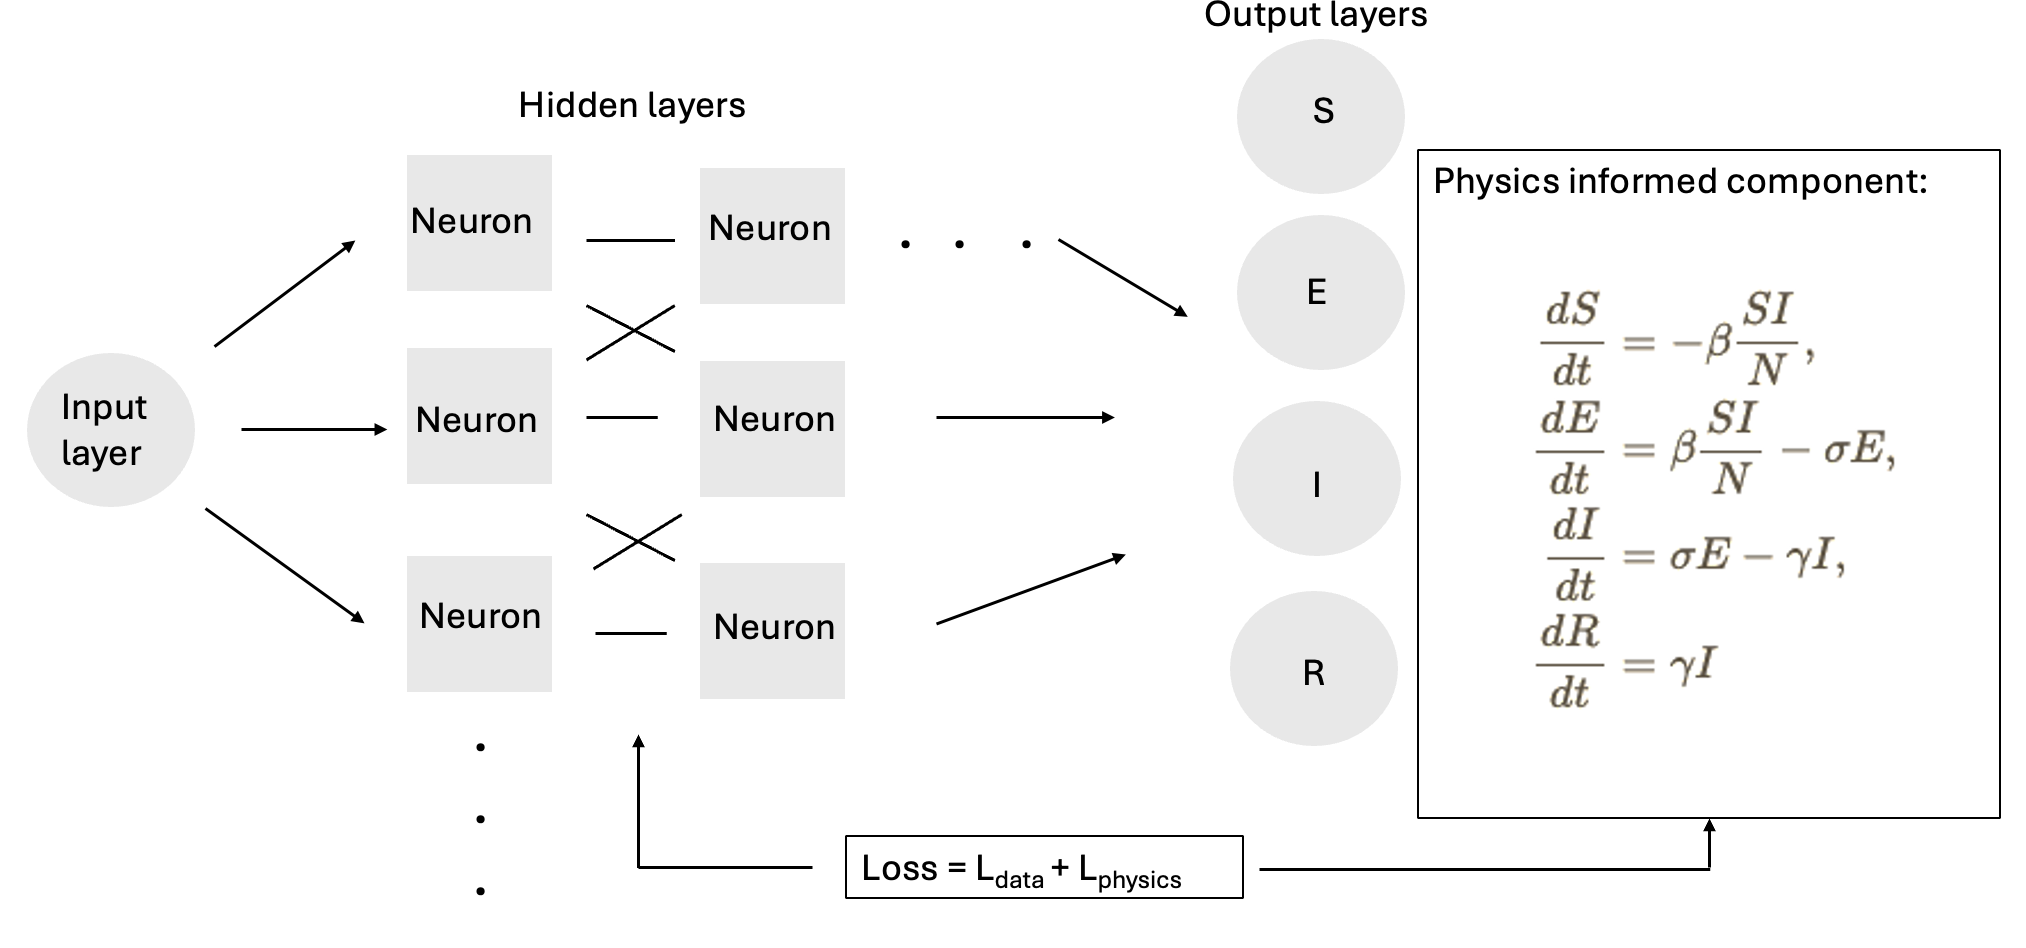
\includegraphics[width=1\linewidth]{figures/Schematic.png}
    \caption{Schematic of a physics informed neural network. The susceptible, exposed, infected, recovered (SEIR) model is embedded into the loss function of a neural network.}
    \label{fig:PINN schematic}
\end{figure}

\subsection{PINNs for forecasting}
PINNs have previously been applied to forecasting in infectious disease epidemiology. \parencite{Berkhahn2022} developed a PINN for estimating COVID-19 transmission parameters and using these to forecast COVID-19 cases and hospitalisations in Germany. \parencite{Millevoi2024} developed a PINN for short term forecasting COVID-19 Italy using a split training approach, training the PINN on data loss first then physics loss. Five synthetic scenarios were used for validation, followed by COVID-19 forecasting using Italian data. \parencite{Kharazmi2021} applied PINNs to a range of epidemiological ODE models, both integer order (the rate of change is dependent on the current state of the system) and fractional order (the rate of change depends on entire history of the system) and time-delay variants to forecast COVID-19 across New York, Rhode Island, Michigan and Italy, with uncertainty quantification included in forecasts. \parencite{https://doi.org/10.48550/arxiv.2506.03897} trained a PINN on synthetic data and used to forecast Influenza cases in Italy, accounting for uncertainty. 

Other PINN models used for infectious disease forecasting have focused on integrating data from diverse sources. \parencite{https://doi.org/10.48550/arxiv.2202.10446}, introduced epidemiology informed neural networks (EINNs) to forecast influenza in US states and health and human services regions. They included a feature model for multi-modal data incorporation, including variables such as mobility and Google symptom survey findings. A recurrent neural network (RNN) was used as the neural network in their model. \parencite{Qian2025} used a PINN to forecast COVID-19 cases, deaths and hospitalisations in California, incorporating an ODE model with 9 coupled equations including information on mobility and vaccination.

Incorporation of spatial structure in PINNs for infectious disease forecasting has been very limited. \parencite{Madden2024} developed a PINN for forecasting measles in England and Wales accounting for measles incidence in the 10 nearest towns and cities. However, they stated that their model could be extended to incorporate a gravity model which incorporates distance and population size into the loss function. Overall, the application of PINNs to spatiotemporal forecasting of infectious disease remains in it's infancy, and further methodological development is needed to account for complex spatiotemporal dependencies in data. The first aim of this project is therefore to develop a spatiotemporal PINN. This could be done using a PINN informed by a metapopulation model, graph neural network (GNN) or partial differential equations (PDEs). 

\subsection{Other mechanistic informed AI/ML methods for forecasting}
While physics informed spatiotemporal machine learning approaches for infectious disease prediction exist, they treat spatial coupling as a data driven quantity rather than encoding it into the model by mechanistic modelling. \parencite{https://doi.org/10.48550/arxiv.2411.17372} developed Heat-GNN, incorporating a time-varying SIR model into a GNN. However, spatial structure was encoded as similarity between regions rather than movement of people/importation of infections. \parencite{https://doi.org/10.48550/arxiv.2410.00049} developed EARTH, epidemiology aware neural ODE, which couples locations through learnt edge weights rather than a mechanistically defined importation term. \parencite{Wang2022} develop causal GNN, which encodes spatial structure as learnt GNN attention rates.

PINNs are adept at handling sparse and noisy data, a feature not seen in models such as graph neural networks (GNNs). GNNs require lots of training data \parencite{Liu2024}. Additionally, methods such as epidemiology informed GNNs don't allow for parameter reconstruction or counterfactual scenario modelling. The closest paper to the best of our knowledge is MepoGNN which incorporates graph neural networks into a metapopulation SIR model. However, the ODE residual is not used as a loss term (ODEs are put into the model). Therefore, the model being proposed is likely to be stronger in sparse/noisy data scenarios and MepoGNN can't be used for counterfactual scenario modelling.

\subsection{PINN for transmission rate parameter reconstruction}
Additionally, the second aim of this project is to reconstruct the transmission rate parameter from the SEIR model. Existing PINNs that recover the transmission rate parameter have relied on observing multiple compartments or have made simplifying assumptions that limit their usefulness. For example, \parencite{https://doi.org/10.48550/arxiv.2510.06776} reconstructed the transmission rate by observing the infected compartment, using recovery periods to model transitions into the recovered compartment, and incorporating total population size. Other studies have recovered constant transmission rates. \parencite{https://doi.org/10.48550/arxiv.2506.03897} used Markov chain Monte Carlo (MCMC) to identify parameters that make the PINN fit the data best. However, they assumed transmission rate to be a scalar constant, therefore not accounting for dynamic changes in transmission. Additionally, they had difficulty in recovering the transmission rate at the start of the outbreak, when cases were low. \parencite{Qian2025} found that despite the PINN making reliable predictions for variables, it could not infer the transmission rate parameter. This project therefore aims to recover a time-varying transmission rate from data using PINNs.

\subsection{Bayesian physics informed neural networks (B-PINNs)}
Another aim of the project is to incorporate uncertainty quantification into the PINNs by developing Bayesian PINNs \parencite{https://doi.org/10.48550/arxiv.2205.08304, https://doi.org/10.48550/arxiv.2003.06097}. Real world infection data are noisy and incomplete, having high amounts of aleatoric uncertainty (uncertainty due to randomness in the data). Uncertainty also arises from model development, epistemic uncertainty \parencite{https://doi.org/10.48550/arxiv.1910.09457}. Uncertainty quantification has persistently been identified as a vital component of model development for policy \parencite{McCabe2021, Zelner2021, Juul2020}, therefore, it is important that a quantification of uncertainty is provided. Bayesian PINNs (B-PINNs) combine PINNs with Bayesian inference, providing probability distributions over neural network parameters. The stochastic neural network (i.e. neural network with stochastic weights) is trained using Bayesian inference \parencite{https://doi.org/10.48550/arxiv.2007.06823}.

\section{Methods}
\subsection{Synthetic data generation: SEIR compartmental model}
Synthetic data was generated using a SEIR compartmental model defined by a system of ODEs (see equations below). The SEIR model in this study is a closed population with no vital dynamics (births or deaths). The SEIR model was solved numerically using \texttt{SciPy solve\_ivp} (SciPy version 1.15.3) using the Runge Kutta method. 

\begin{align}
\frac{dS}{dt} &= -\beta \frac{S I}{N} \\
\frac{dE}{dt} &= \beta \frac{S I}{N} - \sigma E \\
\frac{dI}{dt} &= \sigma E - \gamma I \\
\frac{dR}{dt} &= \gamma I
\end{align}

 The transmission rate parameter ($\beta$) was varied across a range from 0.4 to 0.75. The recovery rate ($\gamma$) was 0.25 and the incubation rate ($\sigma$) was 0.25, corresponding to a mean infectious period and mean incubation period of 4 days.. The model was simulated for a default period of 100 days. Prior to exporting the data, the model outputs were normalised by dividing each compartment (S, E, I, R) by the total population size (N), ensuring all values were between 0 and 1. Additionally, time was rescaled from 0 to 1. 

 In other scenarios, $\beta$ was also varied over time using a variety of cubic splines constructed using the \texttt{Patsy} package in Python \parencite{Hastie2009-iz}.

Additionally, gaussian observation noise was added to models after simulation. Gaussian observation noise was added to the infected compartment with noise levels ranging from 1\% to 20\%.

\subsection{Real data processing: COVID-19 case data for England from the UK Health Security Agency (UKHSA)}
The UK COVID-19 UKHSA case data was imported into Python and filtered to cover England only. Then, a 7-day rolling average was taken and the case data was converted into a population fraction. The data was filtered to include cases from July 2020 to April 2022. Time was normalised [0,1]. 

The PINN was trained using data from July 2020 to April 2022 using a rolling window approach. The PINN was trained on weeks 1 - 17 with predictions for weeks 18 - 21. The training window was then shifted by one week, retraining the model from weeks 1 - 18 and forecasting weeks 19 - 22. This was repeated until predictions were made for weeks 90 - 93. This follows the protocol used in \parencite{Qian2025}.

\subsection{Physics informed neural network (PINN)}
In this study, a PINN framework was applied to SEIR data. The SEIR equations were embedded into the loss function of the neural network. The network was trained to infer the transmission rate and forecast future infection cases. In some scenarios, all the epidemiological parameters and initial conditions were assumed to be known and provided as fixed inputs (\cref{tab:model_parameters}), in others, the network had to learn the transmission and recovery rates. N (the total population) is provided to the PINN in all scenarios.


\begin{table}[h]
    \centering
    \caption{Model parameters used}
    \label{tab:model_parameters}
    
    \begin{tabular}{lll}
        \hline
        Name & Definition & Value \\
        \hline
        $\beta$  & Transmission rate & Estimated by model \\
        $N$      & Population size   & 100001 \\
        $\sigma$ & Incubation rate   & 0.25 \\
        $\gamma$ & Recovery rate     & 0.25 \\
        \hline
    \end{tabular}
\end{table}

The PINN architecture used in this study consists of a simple feedforward neural network (FFNN), specifically, a multi-layer perceptron \parencite{Rumelhart1986} with 3 hidden layers with 50 neurons for the SEIR model and a seperate subnetwork with 3 hidden layers with 50 neurons for the transmission rate parameter ($\beta$). For activation functions, tanh was used for the hidden SEIR and $\beta$ layers and softplus was used for the SEIR output layers, ensuring the values could not be greater than 1 \parencite{Dubey2022}, as was done in \parencite{https://doi.org/10.48550/arxiv.2506.03897}(\cref{tab:model_parameters}). 

The loss function consisted of data loss, physics loss (ODE loss), conservation loss (constraining S + E + I + R to equal 1) and initial condition (IC) loss:

\begin{equation}
L = L_\text{data} + L_\text{ODE} + L_\text{conservation} + L_\text{IC}
\end{equation}

There are 4 output layers for the SEIR model (one layer for susceptible, one layer for exposed, one layer for infected and one layer for recovered) each with one neuron, and one output layer for $\beta$ with one neuron. The model architecture is summarised in (\cref{tab:PINN_architecture}). L2 regularisation was applied to hidden layers to prevent overfitting and penalise large parameter values as in \parencite{Qian2025} \parencite{https://doi.org/10.48550/arxiv.1205.2653}. L2 regularisation was applied as 1 x 10-5.

\begin{table}[h]
    \centering
    \caption{Architecture of the PINN}
    \label{tab:PINN_architecture}
    \begin{tabular}{llll}
        \toprule
        Layer & Type & Size & Activation \\
        \midrule
        Input & Input & 1 & none \\
        Hidden 1 (SEIR) & Dense & 50 & tanh \\
        Hidden 2 (SEIR) & Dense & 50 & tanh \\
        Hidden 3 (SEIR) & Dense & 50 & tanh \\
        Output S & Dense & 1 & softplus \\
        Output E & Dense & 1 & softplus \\
        Output I & Dense & 1 & softplus \\
        Output R & Dense & 1 & softplus \\
        Hidden 1 ($\beta$) & Dense & 50 & tanh \\
        Hidden 2 ($\beta$) & Dense & 50 & tanh \\
        Hidden 3 ($\beta$) & Dense & 50 & tanh \\
        ($\beta$) & Dense & 1 & none \\
        \bottomrule
    \end{tabular}
\end{table}

The loss function gradients were calculated using automatic differentiation via TensorFlows \texttt{gradienttape} (TensorFlow version 2.15.0). The Adam optimiser was used with a learning rate of 0.001 \parencite{https://doi.org/10.48550/arxiv.1412.6980}. Physics loss was evaluated at 1000 evenly distributed collocation points. The PINN was trained in TensorFlow. TensorFlow was used due to having advantages over PyTorch for larger scale problems \parencite{bafghi2024comparing}. The PINN was run for 50,000 iterations, consistent with \parencite{Qian2025}. MSE was used as the loss function.

\begin{equation}
\mathrm{MSE}=\frac{1}{n}\sum_{i=1}^{n}(y_i-\hat{y}_i)^2
\end{equation}

\subsection{Synthetic data generation: metapopulation model}
A metapopulation model was developed to generate synthetic spatial infectious disease outbreak data. This metapopulation model was based on the SEIR model defined previously. Five patches were simulated with 50,000 people in each patch. The infection is seeded with one infected individual in patch 1, with all other patches initialised with fully susceptible populations. The transmission rate for each patch varied from 0.6 - 0.8.  The recovery rate ($\gamma$) was 0.25 and the incubation rate ($\sigma$) was 0.25, corresponding to a mean infectious period and mean incubation period of 4 days.

The force of infection for patch $i$ is defined as:

\begin{equation}
    \lambda_i(t) = \frac{\beta_i I_i(t)}{N_i}
\end{equation}


For each patch $i \in \{1, \dots, P\}$, ODEs defining the epidemic dynamics are:

\begin{align}
    \frac{dS_i}{dt} &= -\lambda_i S_i + \sum_{j=1}^{P} M_{ij} S_j \\[6pt]
    \frac{dE_i}{dt} &= \lambda_i S_i - \sigma E_i + \sum_{j=1}^{P} M_{ij} E_j \\[6pt]
    \frac{dI_i}{dt} &= \sigma E_i - \gamma I_i + \sum_{j=1}^{P} M_{ij} I_j \\[6pt]
    \frac{dR_i}{dt} &= \gamma I_i + \sum_{j=1}^{P} M_{ij} R_j
\end{align}

Spatial coupling between patches was introduced via a migration matrix. The simulation was run for 100 days. The results were normalised prior to being exported.

\subsection{Metapopulation PINN}

The PINN architecture that was previously defined (see section 2.3), was adapted to incorporate the metapopulation SEIR model. The PINN took time and patch index as inputs. The PINN handled all patches simultaneously and $\beta$ was inferred per patch.


\subsection{Data and code availability}
The full code can be found at: https://github.com/AmberFEPalmer/PINN). A detailed README is available describing each script. The UKHSA COVID-19 data is publically accessible from this link: \href{}{https://archive.ukhsa-dashboard.data.gov.uk/coronavirus-dashboard/cases.zip}.

\subsection{Evaluation metrics}

To evaluate the performance of the PINN, mean absolute error (as a percentage) was used which calculates the absolute difference between the observed and predicted values:

\begin{equation}
    \text{MAE\%} = \frac{100}{n \bar{y}} \sum_{i=1}^{n} \left| \hat{y}_i - y_i \right|
\end{equation}


\section{Results}

\subsection{PINN forecasting: constant transmission rate, PINN provided with infection data, recovery rate and incubation period}

A range of synthetic datasets were generated using constant transmission rates during the simulation, with values ranging from $\beta$ = 0.75 to $\beta$ = 0.4. The incubation period, $\sigma$, and recovery rate, $\gamma$, were kept constant in all simulations at 0.25. The parameter values correspond to basic reproduction numbers of R = 3, R = 2 and R = 1.6. The generated synthetic SEIR data are shown in (\Cref{fig:syntheticdata}). Synthetic data was used so the PINN could be evaluated under ground truth. The PINN was provided with data on new infected individuals per day, the recovery rate parameter and the incubation period parameter. Under these conditions, the PINN produced reasonably accurate forecasts across all transmission rate scenarios, as shown in (\Cref{fig:Forecastingconstanttransmssion} and (\cref{tab:MAEForecastingconstanttransmssion}). 

\begin{figure}[H]
    \centering
    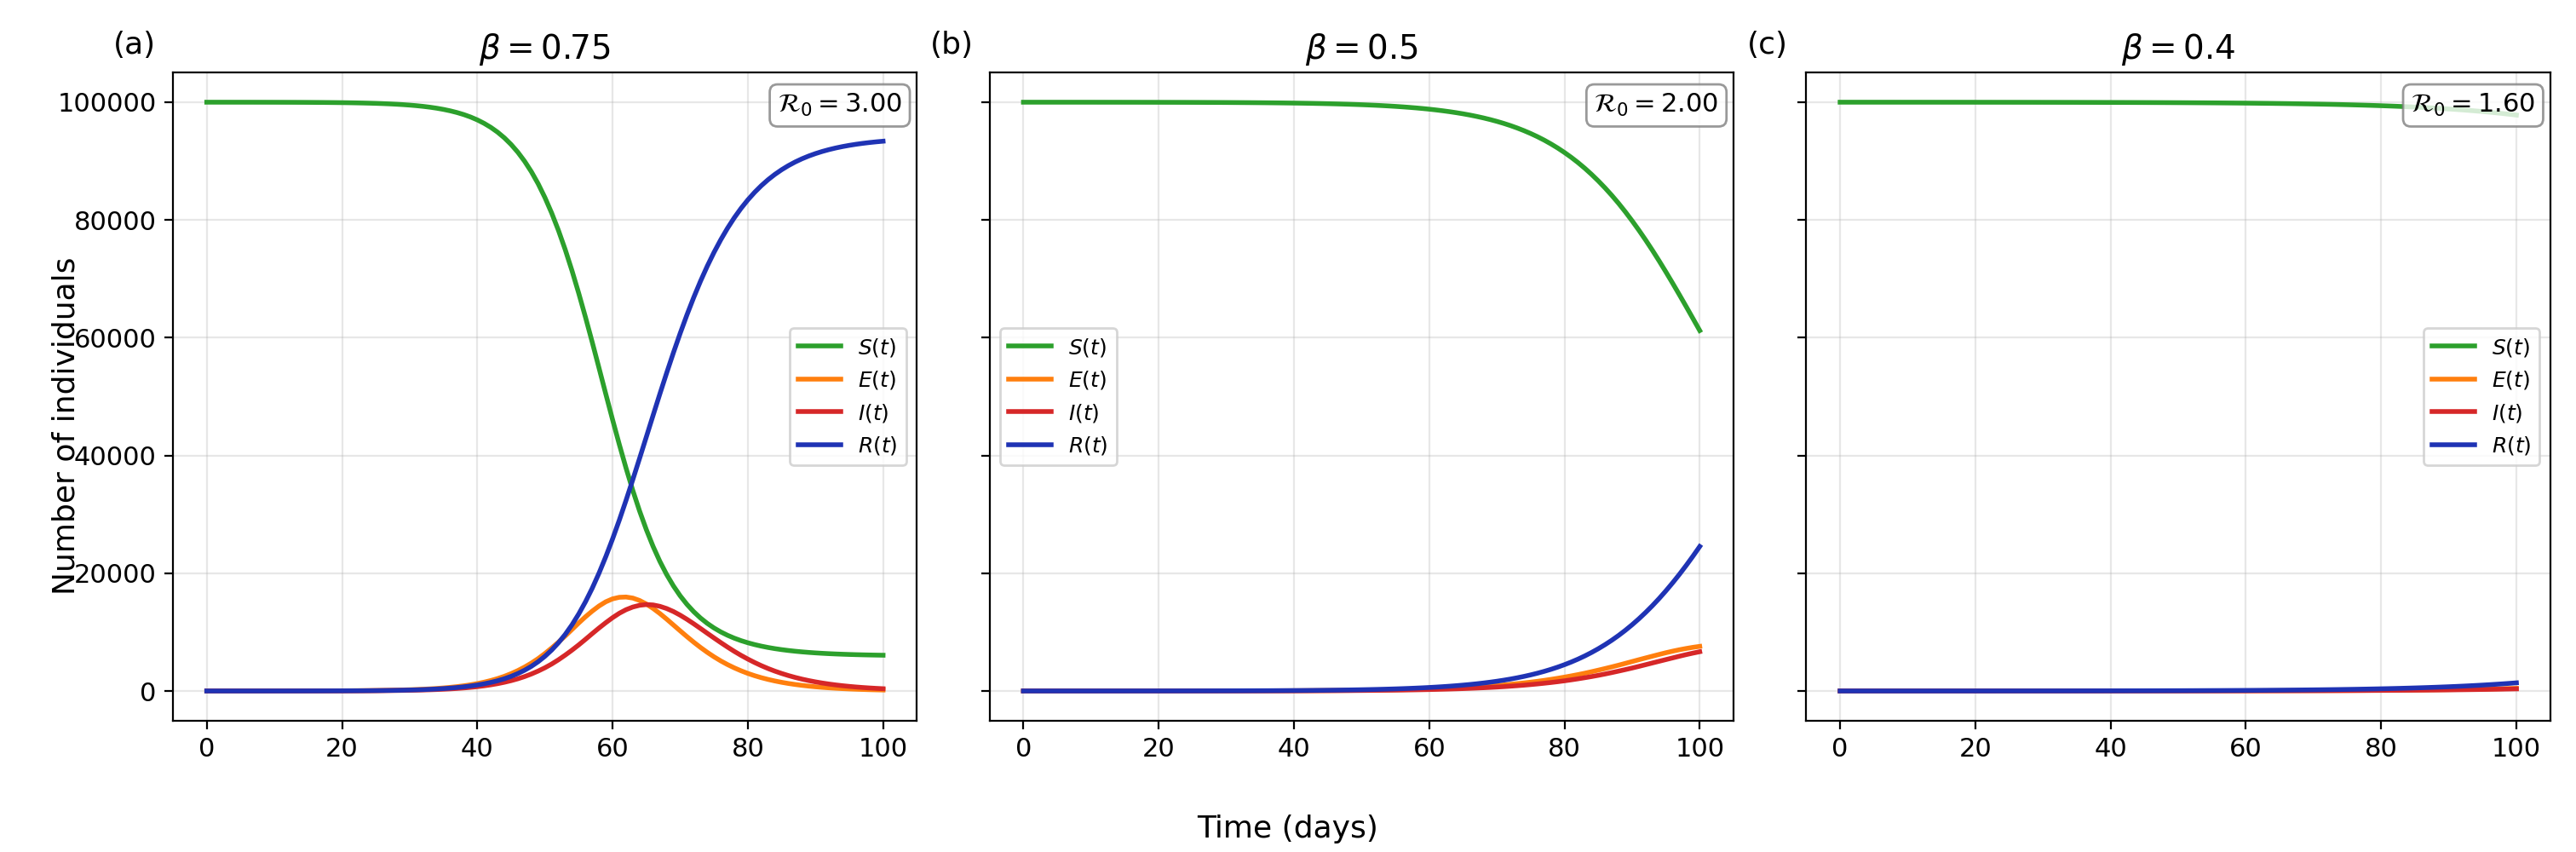
\includegraphics[width=1\linewidth]{figures/Synthetic_data_varying_beta.png}
    \caption{Synthetic data simulations with a constant transmission rate under different parameter values. (b) Results when $\beta$ = 0.75, $\gamma$ = 0.25, $\sigma$= 0.25. (c) Results when $\beta$ = 0.5, $\gamma$ = 0.25, $\sigma$= 0.25. (d) Results when $\beta$ = 0.4, $\gamma$ = 0.25, $\sigma$= 0.25. $\beta$ = transmission rate. $\gamma$ = recovery rate. $\sigma$ = rate of progression from being exposed to the infection and becoming infected (latent period). S = susceptible, E = exposed, I = infected, R = recovered.}
    \label{fig:syntheticdata}
\end{figure}

\begin{figure}[H]
    \centering
    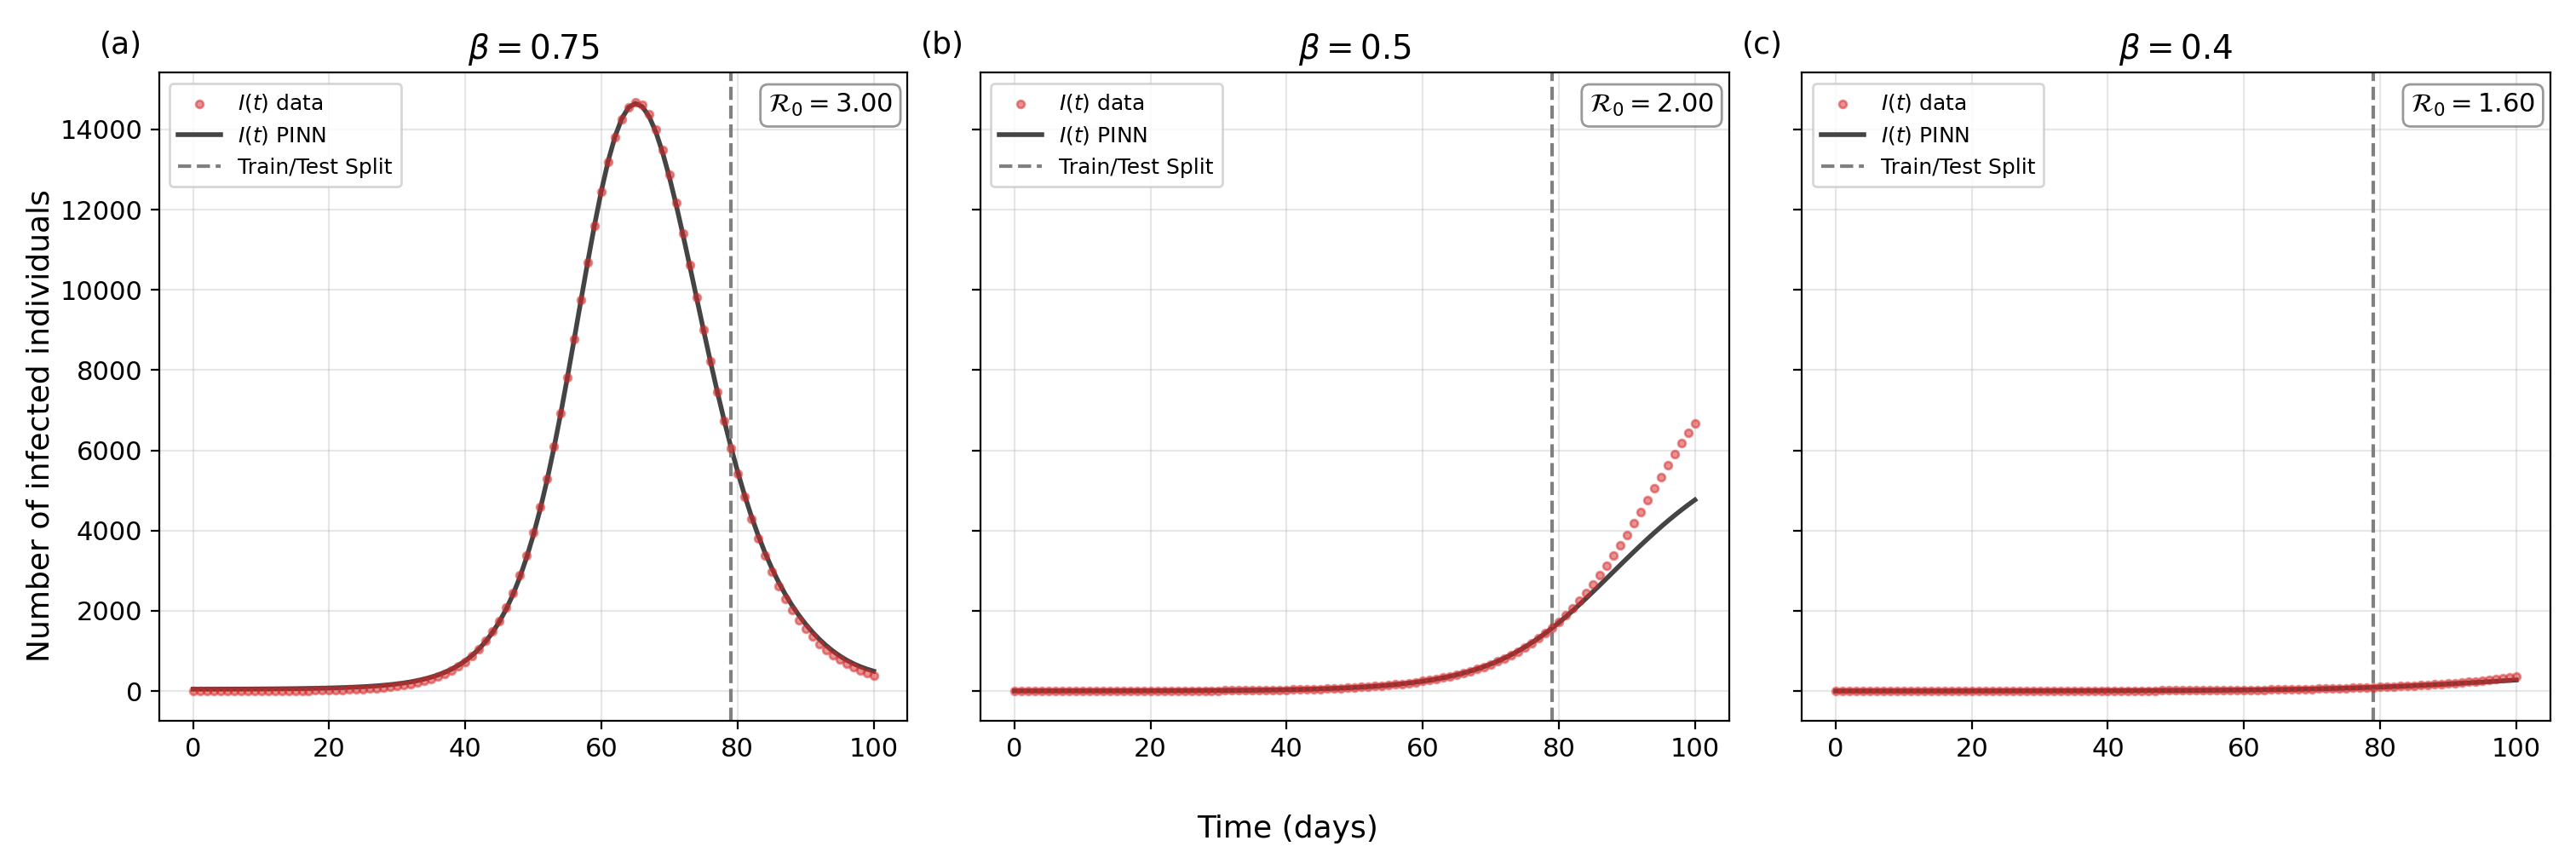
\includegraphics[width=1\linewidth]{figures/PINN_constant_beta.png}
    \caption{Physics informed neural network forecasting on synthetic epidemiological data with a range of parameter values. (a) Forecasting when $\beta$ = 0.75. (b) Forecasting when $\beta$ = 0.5. (c) Forecasting when $\beta$ = 0.4. Only $\beta$ is learnt by the neural network, $\sigma$ and $\gamma$ are fixed at 0.25. The data was split 80\% for training, 20\% for testing.}
    \label{fig:Forecastingconstanttransmssion}
\end{figure}


\begin{table}[H]
    \centering
    \begin{tabular}{llll}
        \hline
        Scenario & Mean absolute error \% (MAE)\\
        \hline
        Infected compartment $\beta = 0.75$ & 1.45\\
        Infected compartment $\beta = 0.5$ & 15.68\\
        Infected compartment $\beta = 0.4$ & 8.92\\
        \hline
    \end{tabular}
    \caption{Mean absolute error for PINN forecasting on synthetic epidemiological data with a range of parameter values. Infection data, recovery rate parameter and incubation rate parameters were provided as inputs to the PINN.}
    \label{tab:MAEForecastingconstanttransmssion}
\end{table}



\subsection{PINN forecasting: constant transmission rate, PINN provided with infection data only}

The PINN was provided with infection data only, i.e. the PINN had to infer the incubation period and recovery period from the data. Under this scenario, the PINN still made accurate forecasts under a range of transmission rate scenarios (\cref{fig:PINN_constant_beta_all_learnable_parameters}) and (\cref{tab:MAEForecastingconstanttransmssionAlllearnable}).

\begin{figure}[H]
    \centering
    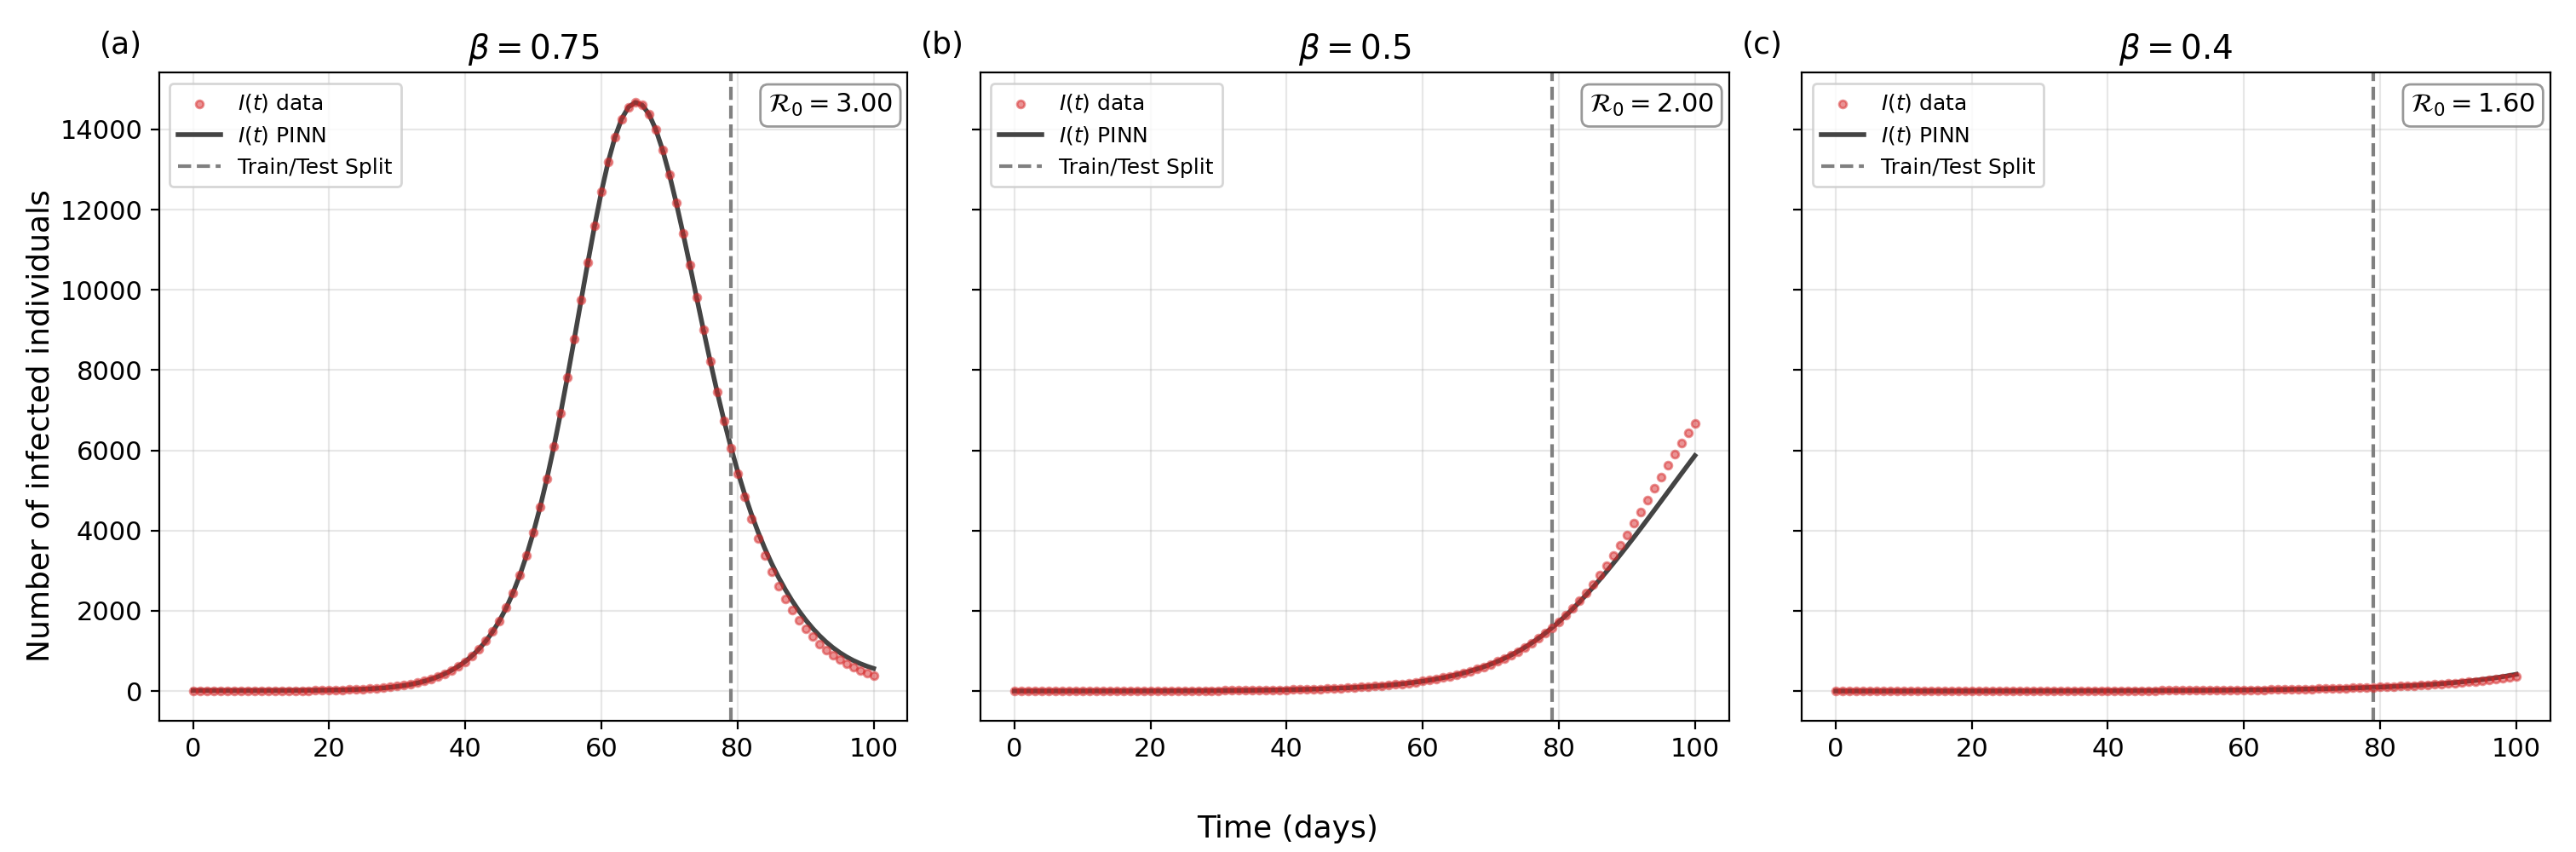
\includegraphics[width=1\linewidth]{figures/PINN_constant_beta_all_learnable_parameters.png}
    \caption{Physics informed neural network forecasting on synthetic epidemiological data with a range of parameter values. (a) Forecasting when $\beta$ = 0.75. (b) Forecasting when $\beta$ = 0.5. (c) Forecasting when $\beta$ = 0.4. $\beta$, $\sigma$ and $\gamma$ are learnt by the neural network. The data was split 80\% for training, 20\% for testing.}
    \label{fig:PINN_constant_beta_all_learnable_parameters}
\end{figure}

\begin{table}[H]
    \centering
    \begin{tabular}{llll}
        \hline
        Scenario & Mean absolute error \% (MAE)\\
        \hline
        Infected compartment $\beta = 0.75$ & 1.19\\
        Infected compartment $\beta = 0.5$ & 7.25\\
        Infected compartment $\beta = 0.4$ & 5.67\\
        \hline
    \end{tabular}
    \caption{Mean absolute error on physics informed neural network forecasting on synthetic epidemiological data with a range of parameter values. Infection data were provided as inputs to the PINN.}
    \label{tab:MAEForecastingconstanttransmssionAlllearnable}
\end{table}

\subsection{PINN transmission rate parameter reconstruction: constant transmission rate, PINN provided with infection data, recovery rate and incubation period}

When the PINN was provided with infection data, the recovery rate parameter and the incubation rate parameter, the PINN could accurately reproduce a constant transmission rate from synthetic SEIR data (\cref{fig:PINN_constant_beta_parameter_reconstruction.pn}). This was the case for all epidemiological scenarios studied with $\beta$ = 0.75, $\beta$ = 0.5, $\beta$ = 0.4.

\begin{figure}[H]
    \centering
    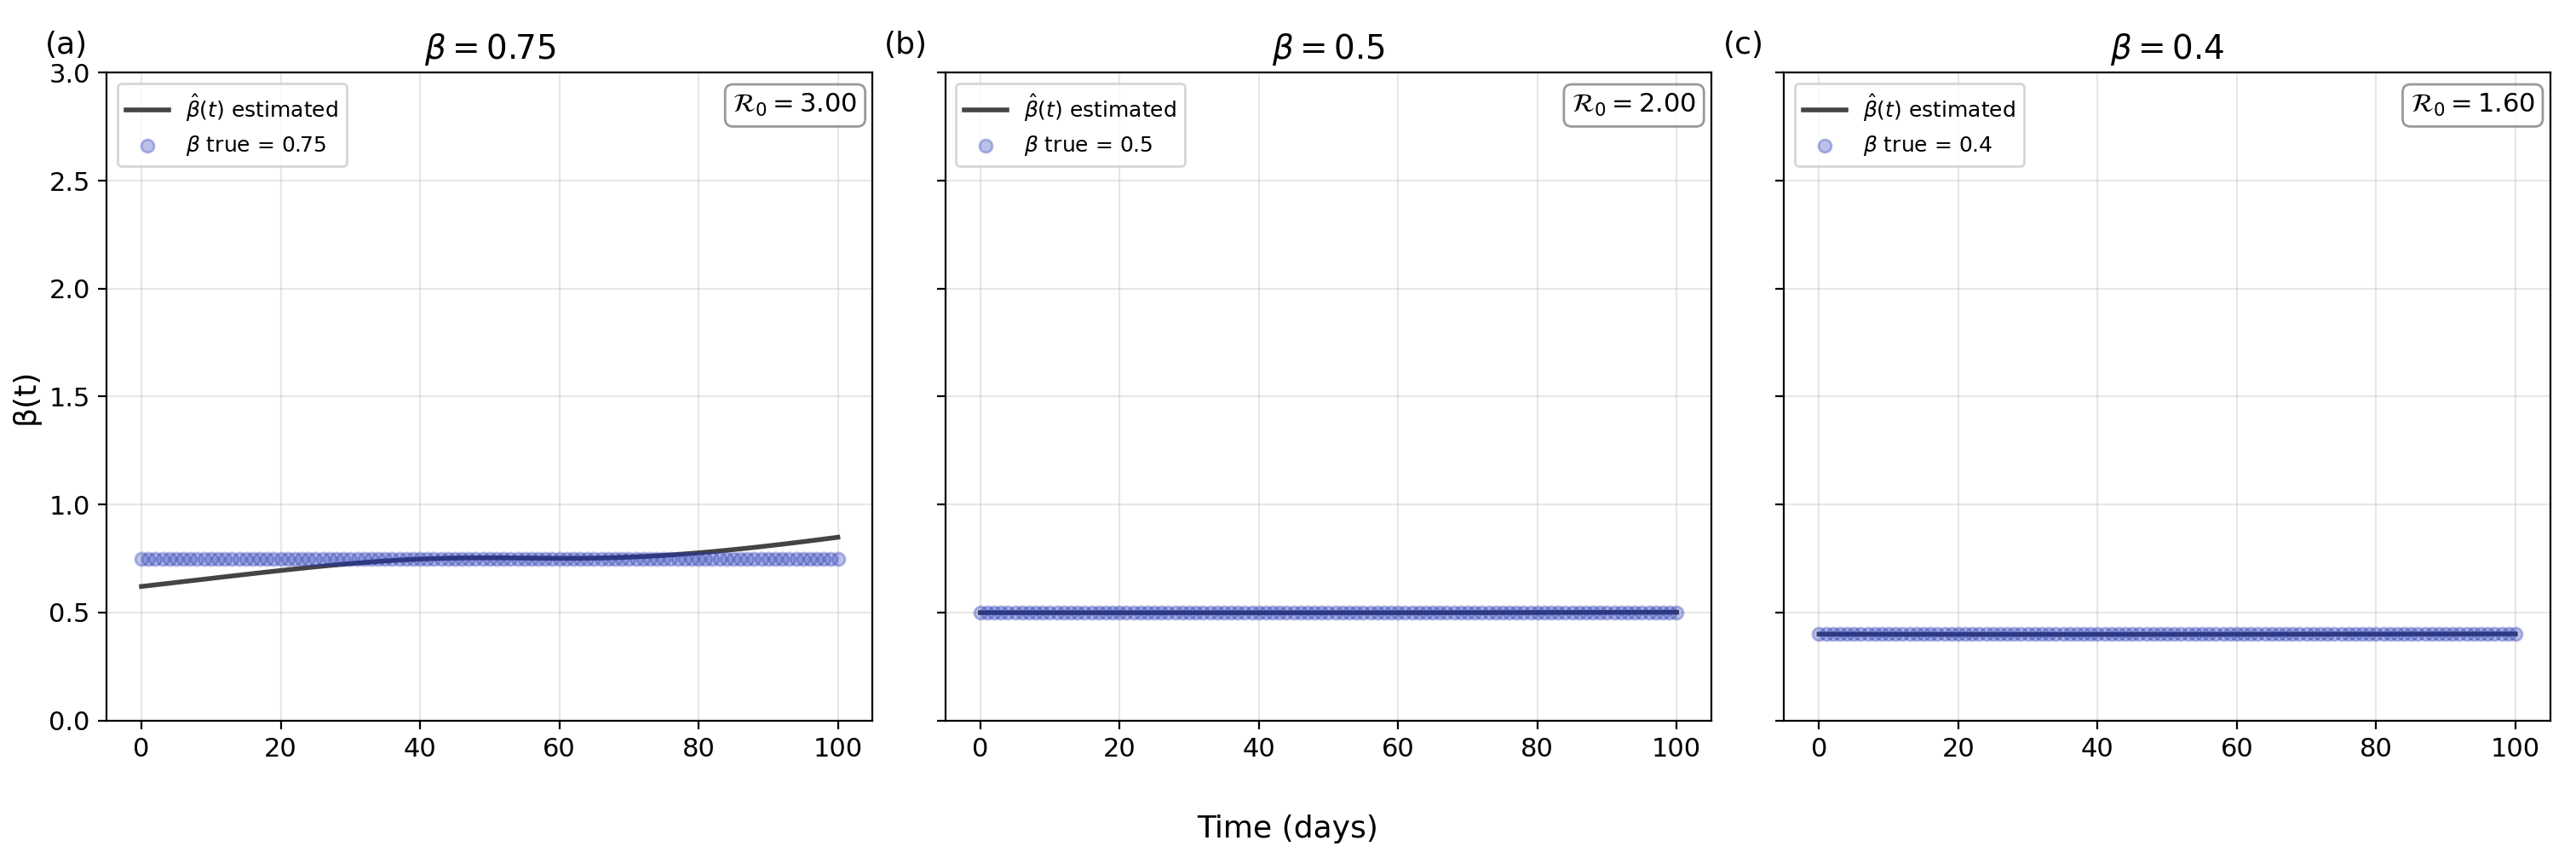
\includegraphics[width=1\linewidth]{figures/PINN_constant_beta_parameter_reconstruction.png}
    \caption{Physics informed neural network transmission rate parameter reconstruction on synthetic epidemiological data with a range of parameter values. (a) Parameter reconstruction when $\beta$ = 0.75. (b) Parameter reconstruction when $\beta$ = 0.5. (c) Parameter reconstruction when $\beta$ = 0.4. $\beta$ is learnt by the neural network, $\sigma$ and $\gamma$ are provided. }
    \label{fig:PINN_constant_beta_parameter_reconstruction.pn}
\end{figure}


\subsection{PINN transmission rate parameter reconstruction: constant transmission rate, PINN provided with infection data only}

The PINN failed to reconstruct constant transmission rate parameter when only infection data was provided, consistently underpredicting the transmission rate parameter (\cref{fig:PINN_constant_beta_parameter_reconstruction_all_learnable_parameters}). In an SEIR model, when only incidence data is given, the transmission rate parameter is structurally unidentifiable \parencite{Dankwa2022, Roda2020, Massonis2021}. This means the failure to reconstruct $\beta$ is not indicative of an error in the model architecture, but rather a property of the SEIR model with the data being provided. Despite the PINN failing to reconstruct the transmission rate, forecasting is still accurate under these conditions. This provides evidence that accurate forecasts can mask the PINN not being able to reconstruct parameter values.

\begin{figure}[H]
    \centering
    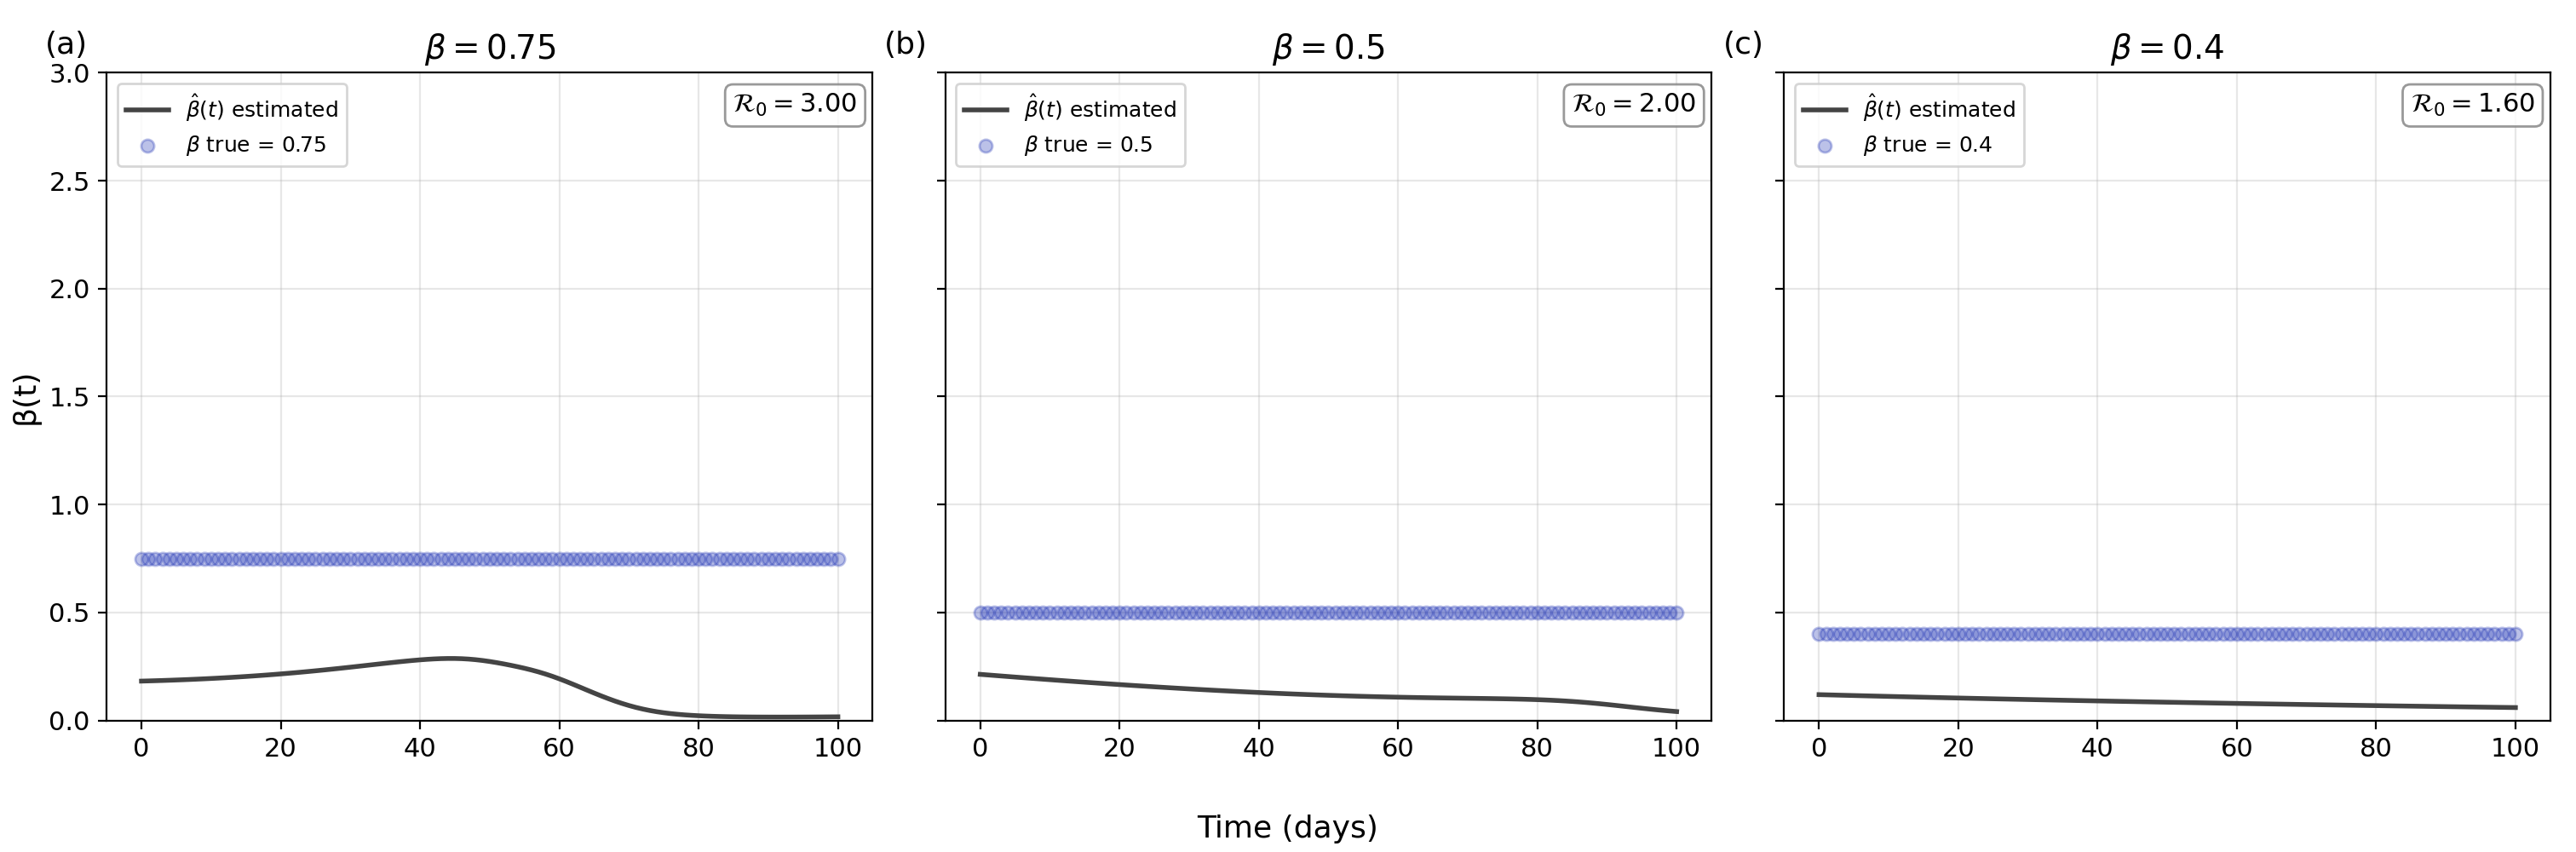
\includegraphics[width=1\linewidth]{figures/PINN_constant_beta_parameter_reconstruction_all_learnable_parameters.png}
    \caption{Physics informed neural network transmission rate parameter reconstruction on synthetic epidemiological data with a range of parameter values. (a) Parameter reconstruction when $\beta$ = 0.75. (b) Parameter reconstruction when $\beta$ = 0.5. (c) Parameter reconstruction when $\beta$ = 0.4. $\beta$, $\sigma$ and $\gamma$ where learnt by the neural network. Only infection data was given. }
    \label{fig:PINN_constant_beta_parameter_reconstruction_all_learnable_parameters}
\end{figure}

\subsection{Synthetic data generation: SEIR model changing beta}

A range of synthetic outbreak scenarios were simulated where $\beta$ changed over time were developed. $\beta$ varying over time was modelled as variations of cubic splines. Scenarios ranged from simple changes over time e.g. slow rise in $\beta$ or a gradual decline, to more complex changes such as $\beta$ having rapid oscillations. These scenarios were developed to test how the PINN coped with time-varying transmission rates, as would be seen in a real-world outbreak scenario (\cref{fig:SEIR_changing_beta}).

\begin{figure}[H]
    \centering
    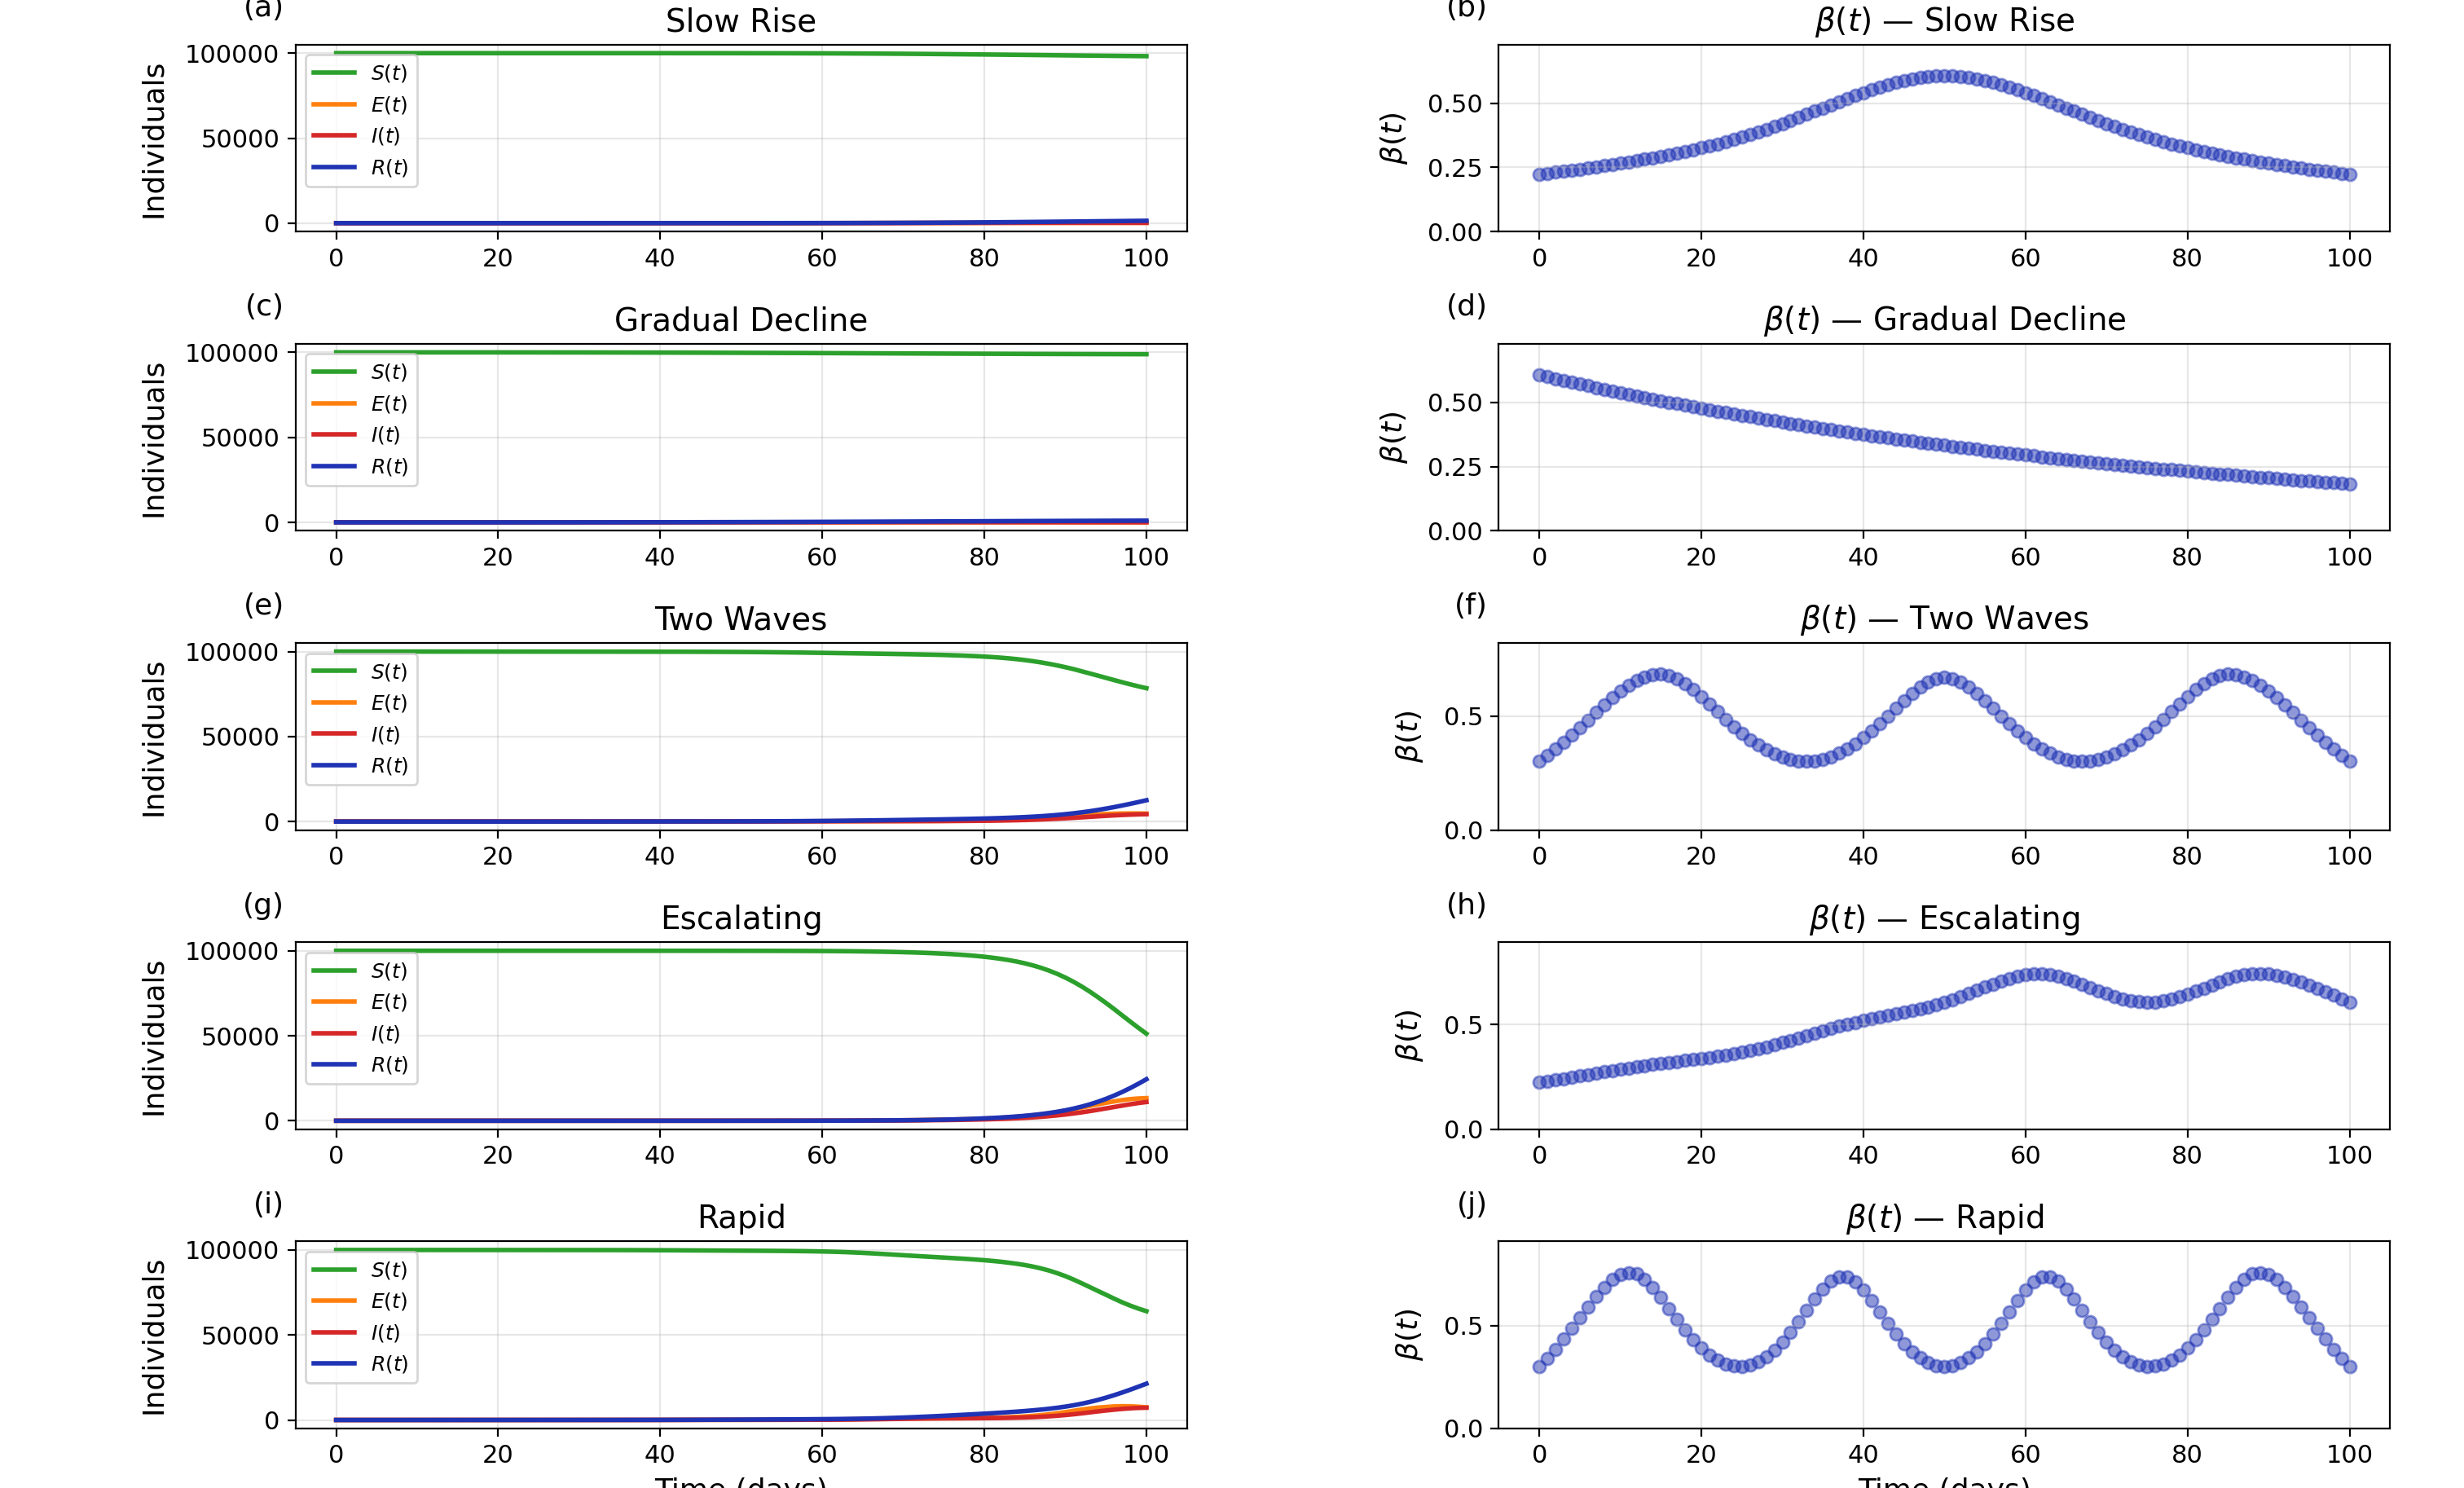
\includegraphics[width=1\linewidth]{figures/SEIR_changing_beta.png}
    \caption{Synthetic SEIR simulations for time varying transmission rate parameter. (a) Susceptible, exposed, infected and recovered individuals during the simulation for the SEIR model when $\beta$ varies as one wave that slowly rises and declines. (b) Values for $\beta$ during the the simulation for the SEIR model when $\beta$ varies as one wave that slowly rises and declines. (c) Susceptible, exposed, infected and recovered individuals during the simulation for the SEIR model when $\beta$ gradually declines during the simulation. (d) Values for $\beta$ during the the simulation for the SEIR model when $\beta$ declines gradually. (e) Susceptible, exposed, infected and recovered individuals during the simulation for the SEIR model when $\beta$ varies as three waves. (f) Values for $\beta$ during the the simulation for the SEIR model when $\beta$ varies as three waves. (g) Susceptible, exposed, infected and recovered individuals during the simulation for the SEIR model when $\beta$ increases during the simulation. (h) Values for $\beta$ during the the simulation for the SEIR model when $\beta$ increases during the simulation. (i) Susceptible, exposed, infected and recovered individuals during the simulation for the SEIR model when $\beta$ oscillates rapidly. (j) Values for $\beta$ during the the simulation for the SEIR model when $\beta$ oscillates rapidly during the simulation.}
    \label{fig:SEIR_changing_beta}
\end{figure}

\subsection{PINN forecasting: time varying transmission rate, PINN provided with infection data, recovery rate and incubation period}

The PINN could provide reasonable forecasts for the easier time varying $\beta$ scenarios such as a single wave or a gradual decline in transmission. However, the PINN struggled as the changes in $\beta$ became more complex i.e. when $\beta$ increased throughout the simulation or when $\beta$ oscillated, greatly underestimating the number of infected individuals (\cref{fig:PINN_forecast_changing_beta}).

\begin{figure}[H]
    \centering
    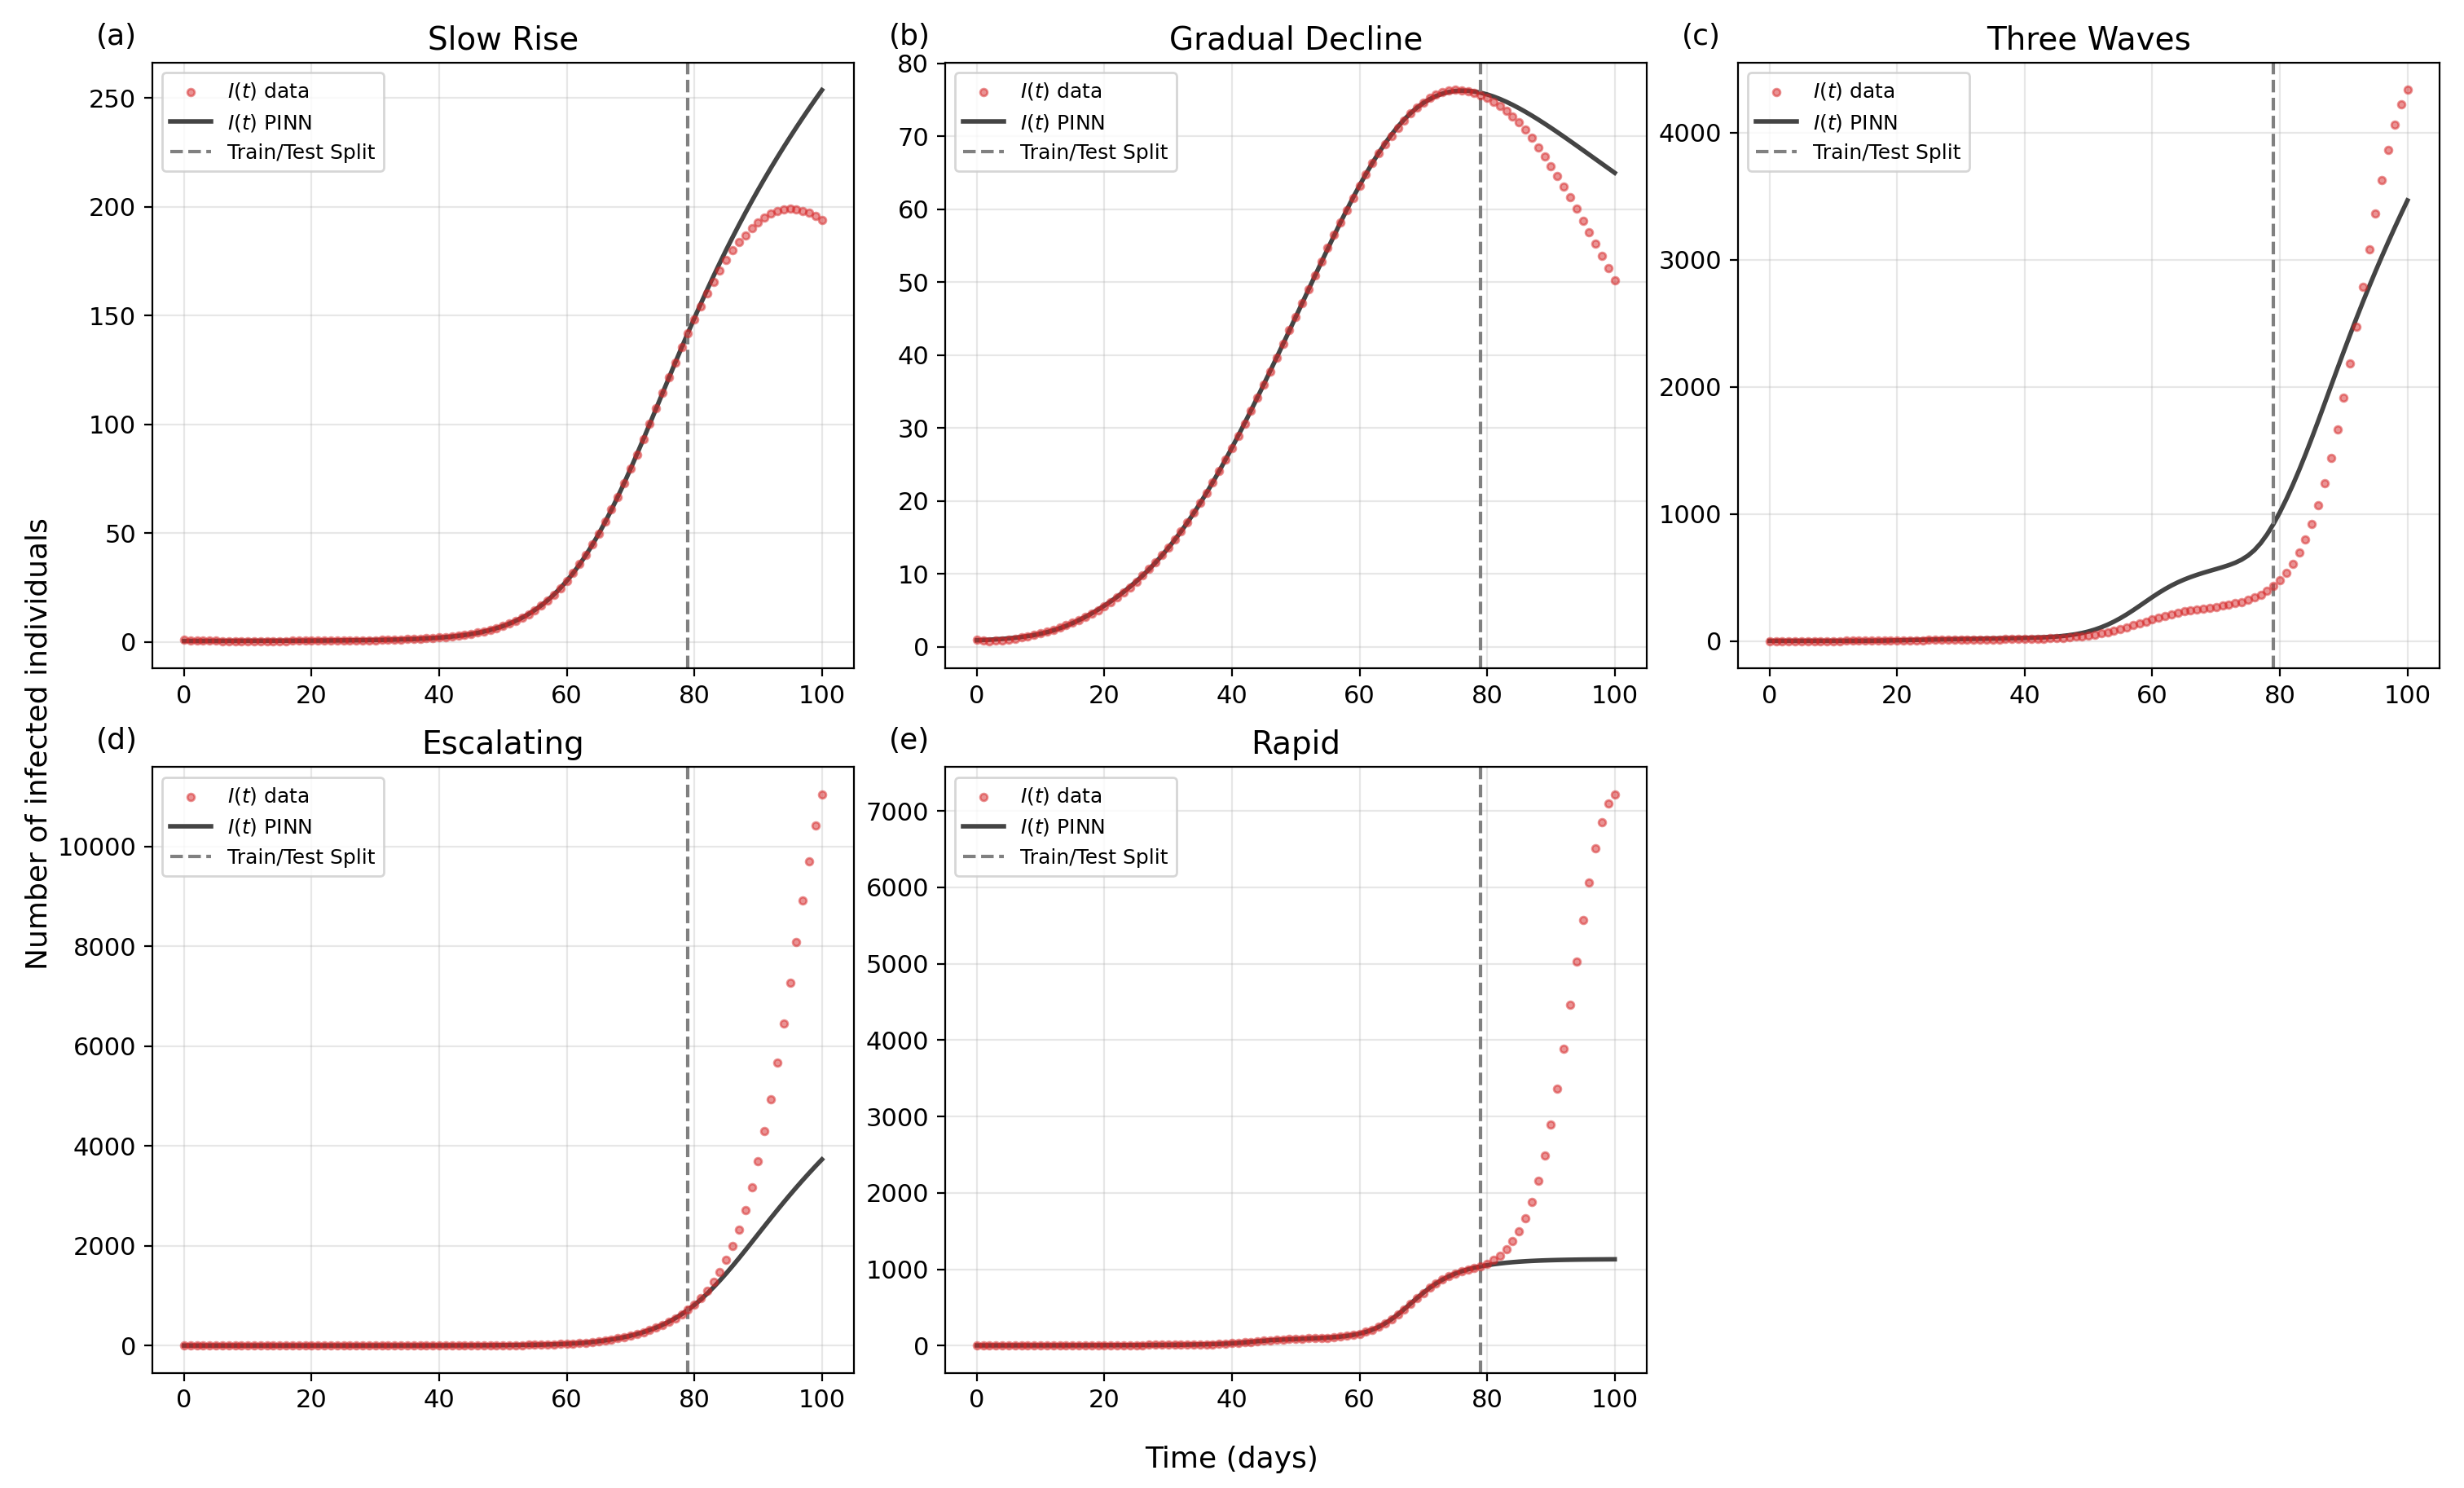
\includegraphics[width=1\linewidth]{figures/PINN_forecast_changing_beta.png}
    \caption{PINN forecasting on a range of time-varying beta transmission rate scenarios. (a) PINN forecasting when $\beta$ changes in the synthetic data as one wave that slowly rises and declines. (b) PINN forecasting when $\beta$ changes in the synthetic data as a gradual decline over time. (c) PINN forecasting when $\beta$ changes in the synthetic data as three waves. (d) PINN forecasting when $\beta$ changes in the synthetic data as increasing over time. (e) PINN forecasting when $\beta$ changes in the synthetic data as rapid oscillations. PINN provided with infection data, recovery rate and incubation period. The data was split 80\% for training, 20\% for testing.}
    \label{fig:PINN_forecast_changing_beta}
\end{figure}

\subsection{PINN forecasting: time varying transmission rate, PINN provided with infection data only}

The PINN was again able to provide reasonable forecasts for the easier time varying $\beta$ scenarios, but struggled as the changes in $\beta$ became more complex (\cref{fig:PINN_forecasting_changing_beta_all_learnable_parameters}).

\begin{figure}[H]
    \centering
    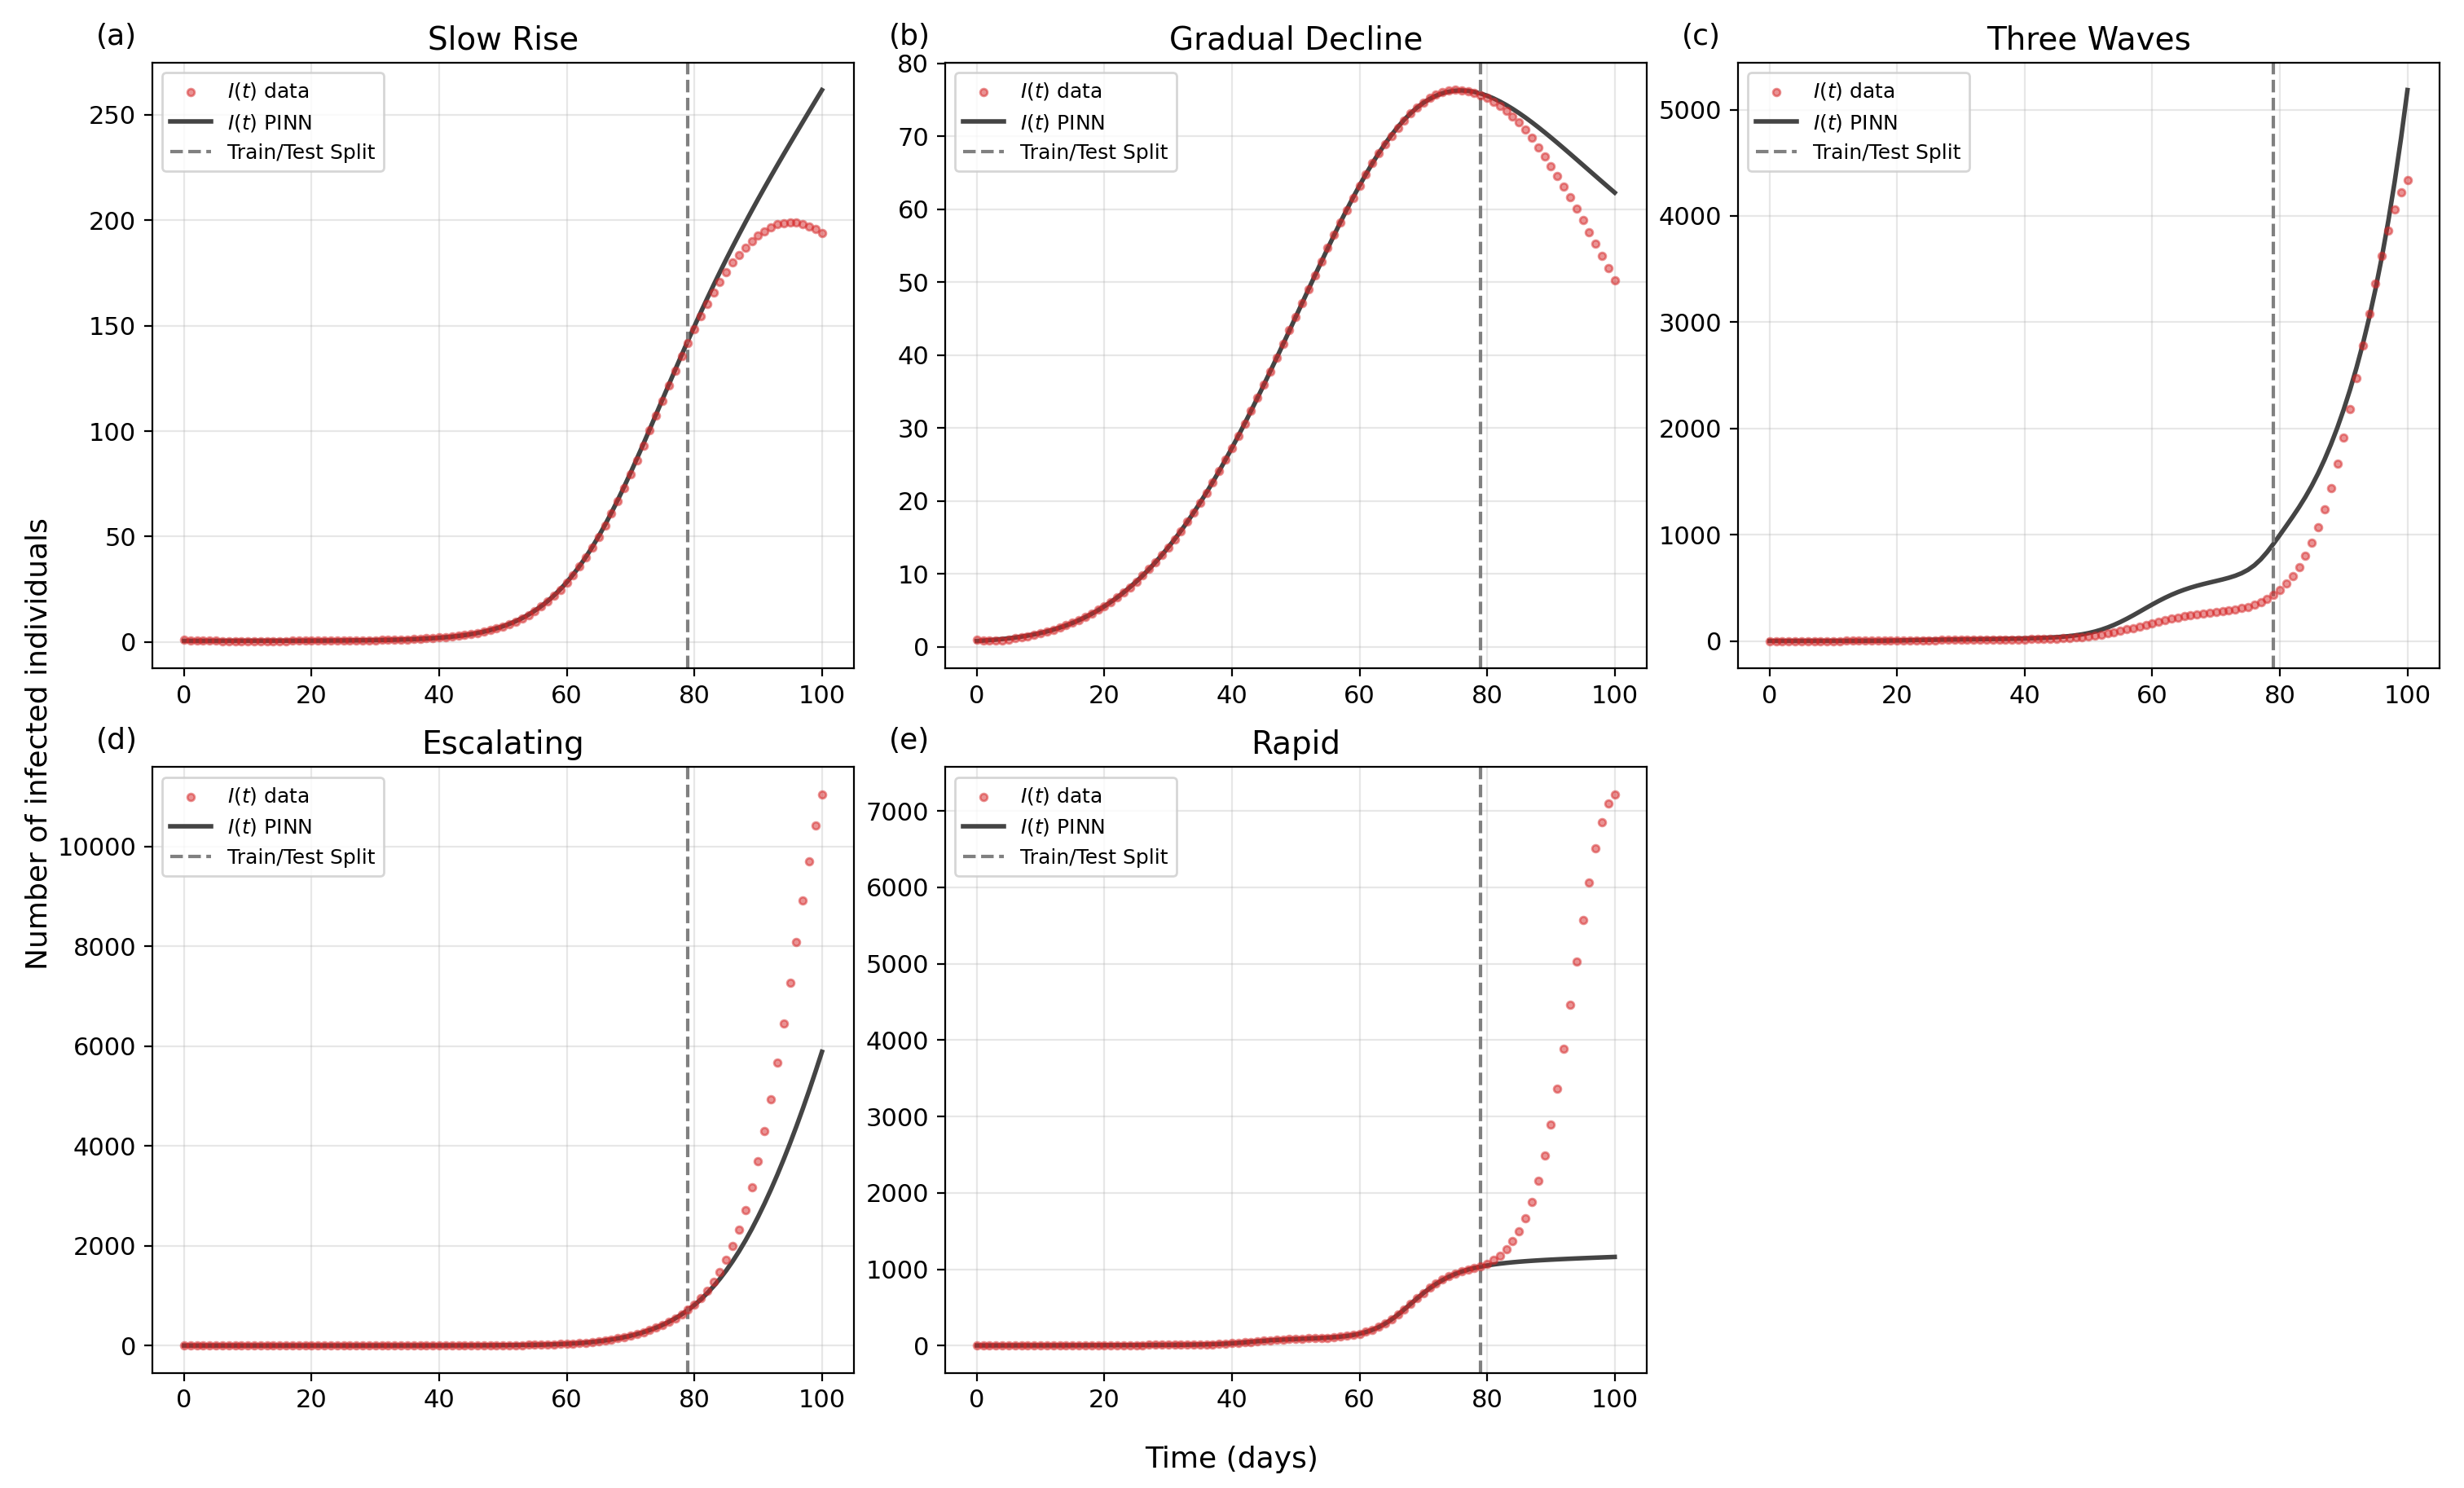
\includegraphics[width=1\linewidth]{figures/PINN_forecasting_changing_beta_all_learnable_parameters.png}
    \caption{PINN forecasting on a range of time-varying beta transmission rate scenarios. (a) PINN forecasting when $\beta$ changes in the synthetic data as one wave that slowly rises and declines. (b) PINN forecasting when $\beta$ changes in the synthetic data as a gradual decline over time. (c) PINN forecasting when $\beta$ changes in the synthetic data as three waves. (d) PINN forecasting when $\beta$ changes in the synthetic data as increasing over time. (e) PINN forecasting when $\beta$ changes in the synthetic data as rapid oscillations. PINN provided with infection data, recovery rate and incubation period. PINN provided with infection data only. The data was split 80\% for training, 20\% for testing.}
    \label{fig:PINN_forecasting_changing_beta_all_learnable_parameters}
\end{figure}


\subsection{PINN parameter reconstruction time varying transmission rate, PINN provided with infection data, recovery rate and incubation period}

The PINN failed to reconstruct $\beta$ in all scenarios except the gradual decline in $\beta$ (\cref{fig:PINN_parameter_estimation_changing_beta}). Because the PINN is being provided with infection data, the recovery rate parameter and the incubation rate parameter, this is likely to be due to the spectral bias of neural networks \parencite{https://doi.org/10.48550/arxiv.2602.19265, https://doi.org/10.48550/arxiv.1806.08734}, i.e. the PINN learns lower frequency solutions before higher frequency solutions, meaning the PINN will recover solutions where $\beta$ is smooth, with time-varying $\beta$ either being learnt slowly or not at all. 

The inability to recover parameters while forecasts still being reasonably accurate also adds to the evidence that accurate PINN forecasting can often mask the PINN not being able to accurately recover parameters. 

\begin{figure}[H]
    \centering
    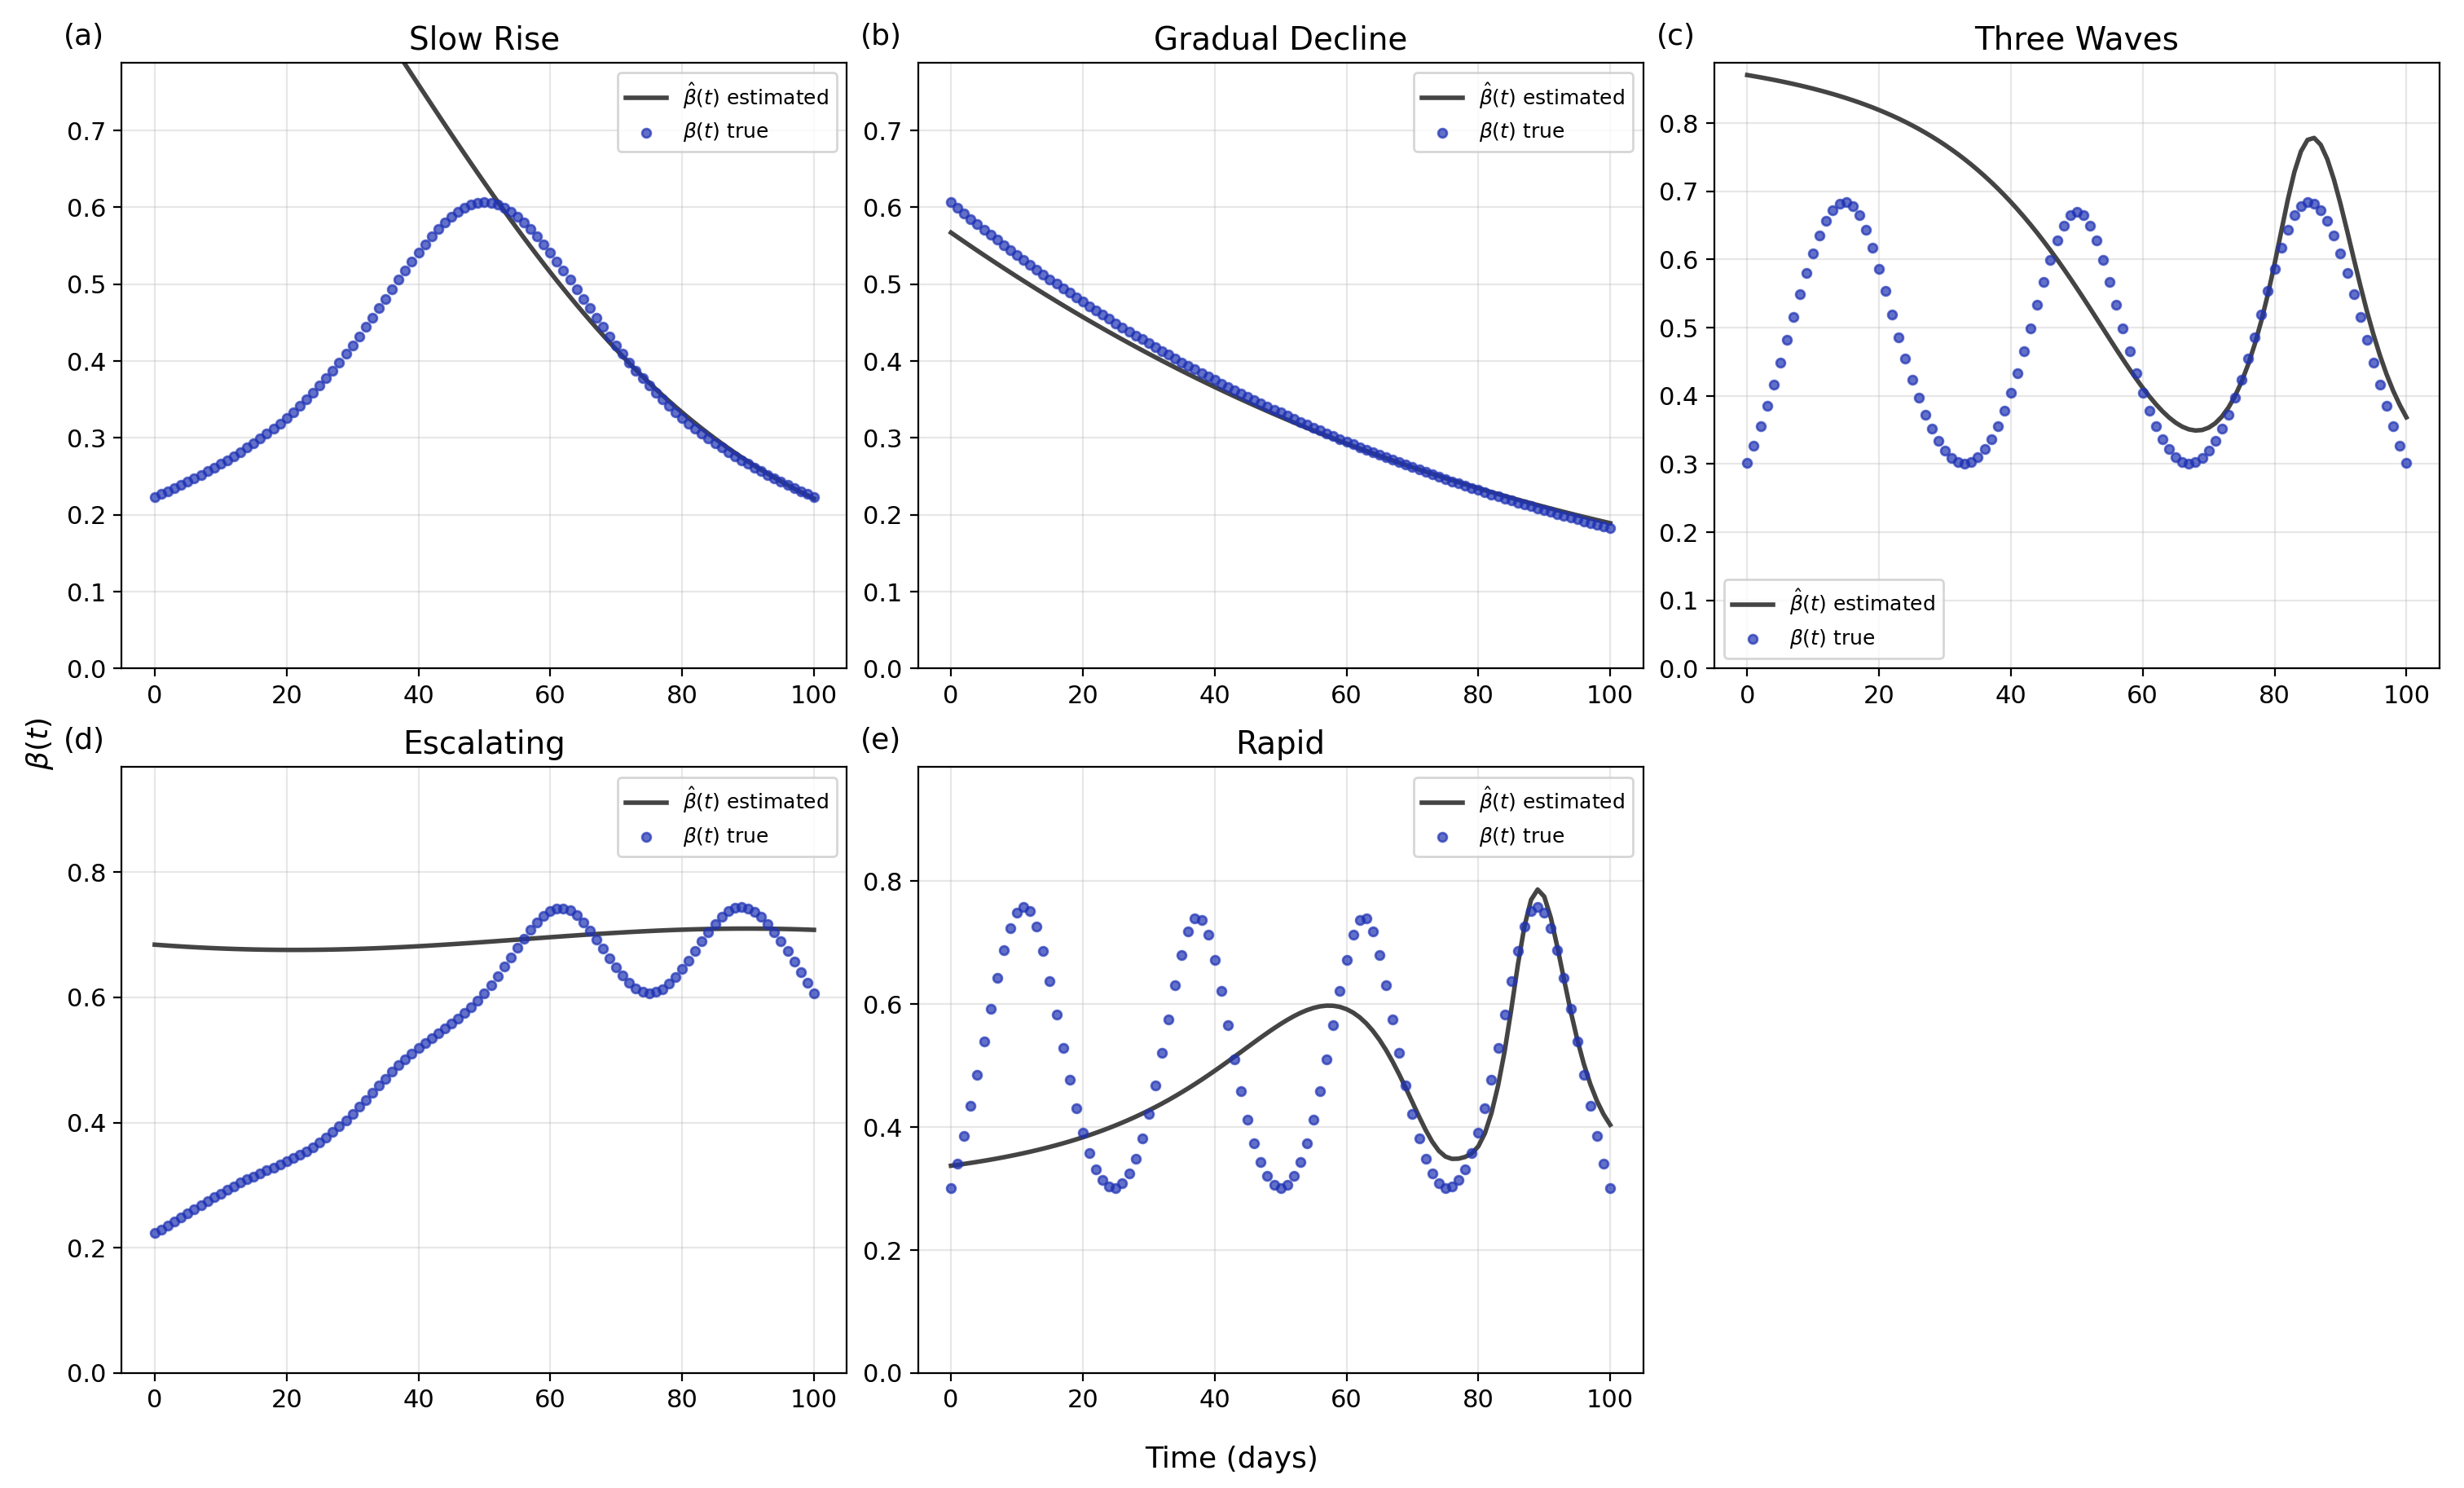
\includegraphics[width=1\linewidth]{figures/PINN_parameter_estimation_changing_beta.png}
    \caption{PINN parameter reconstruction on a range of time-varying beta transmission rate scenarios.
    (a) PINN parameter estimation when $\beta$ changes in the synthetic data as one wave that slowly rises and declines. (b) PINN parameter estimation when $\beta$ changes in the synthetic data as a gradual decline over time. (c) PINN parameter estimation when $\beta$ changes in the synthetic data as three waves. (d) PINN parameter estimation when $\beta$ changes in the synthetic data as increasing over time. (e) PINN parameter estimation when $\beta$ changes in the synthetic data as rapid oscillations. PINN provided with infection data, recovery rate and incubation period.}
    \label{fig:PINN_parameter_estimation_changing_beta}
\end{figure}


\subsection{PINN parameter reconstruction time varying transmission rate, PINN provided with infection data only}
When $\beta$ was time-varying and the PINN was only provided with infection data, the PINN failed at reconstructing parameters for all scenarios of time-varying $\beta$ (\cref{fig:PINN_parameter_estimation_changing_beta_infection_only}). This scenario combines the issues previously highlighted of $\beta$ being structurally unidentifiable when only infection data is provided and the PINN struggling to learn sharp changes in $\beta$ due to it's spectral bias.

\begin{figure}[H]
    \centering
    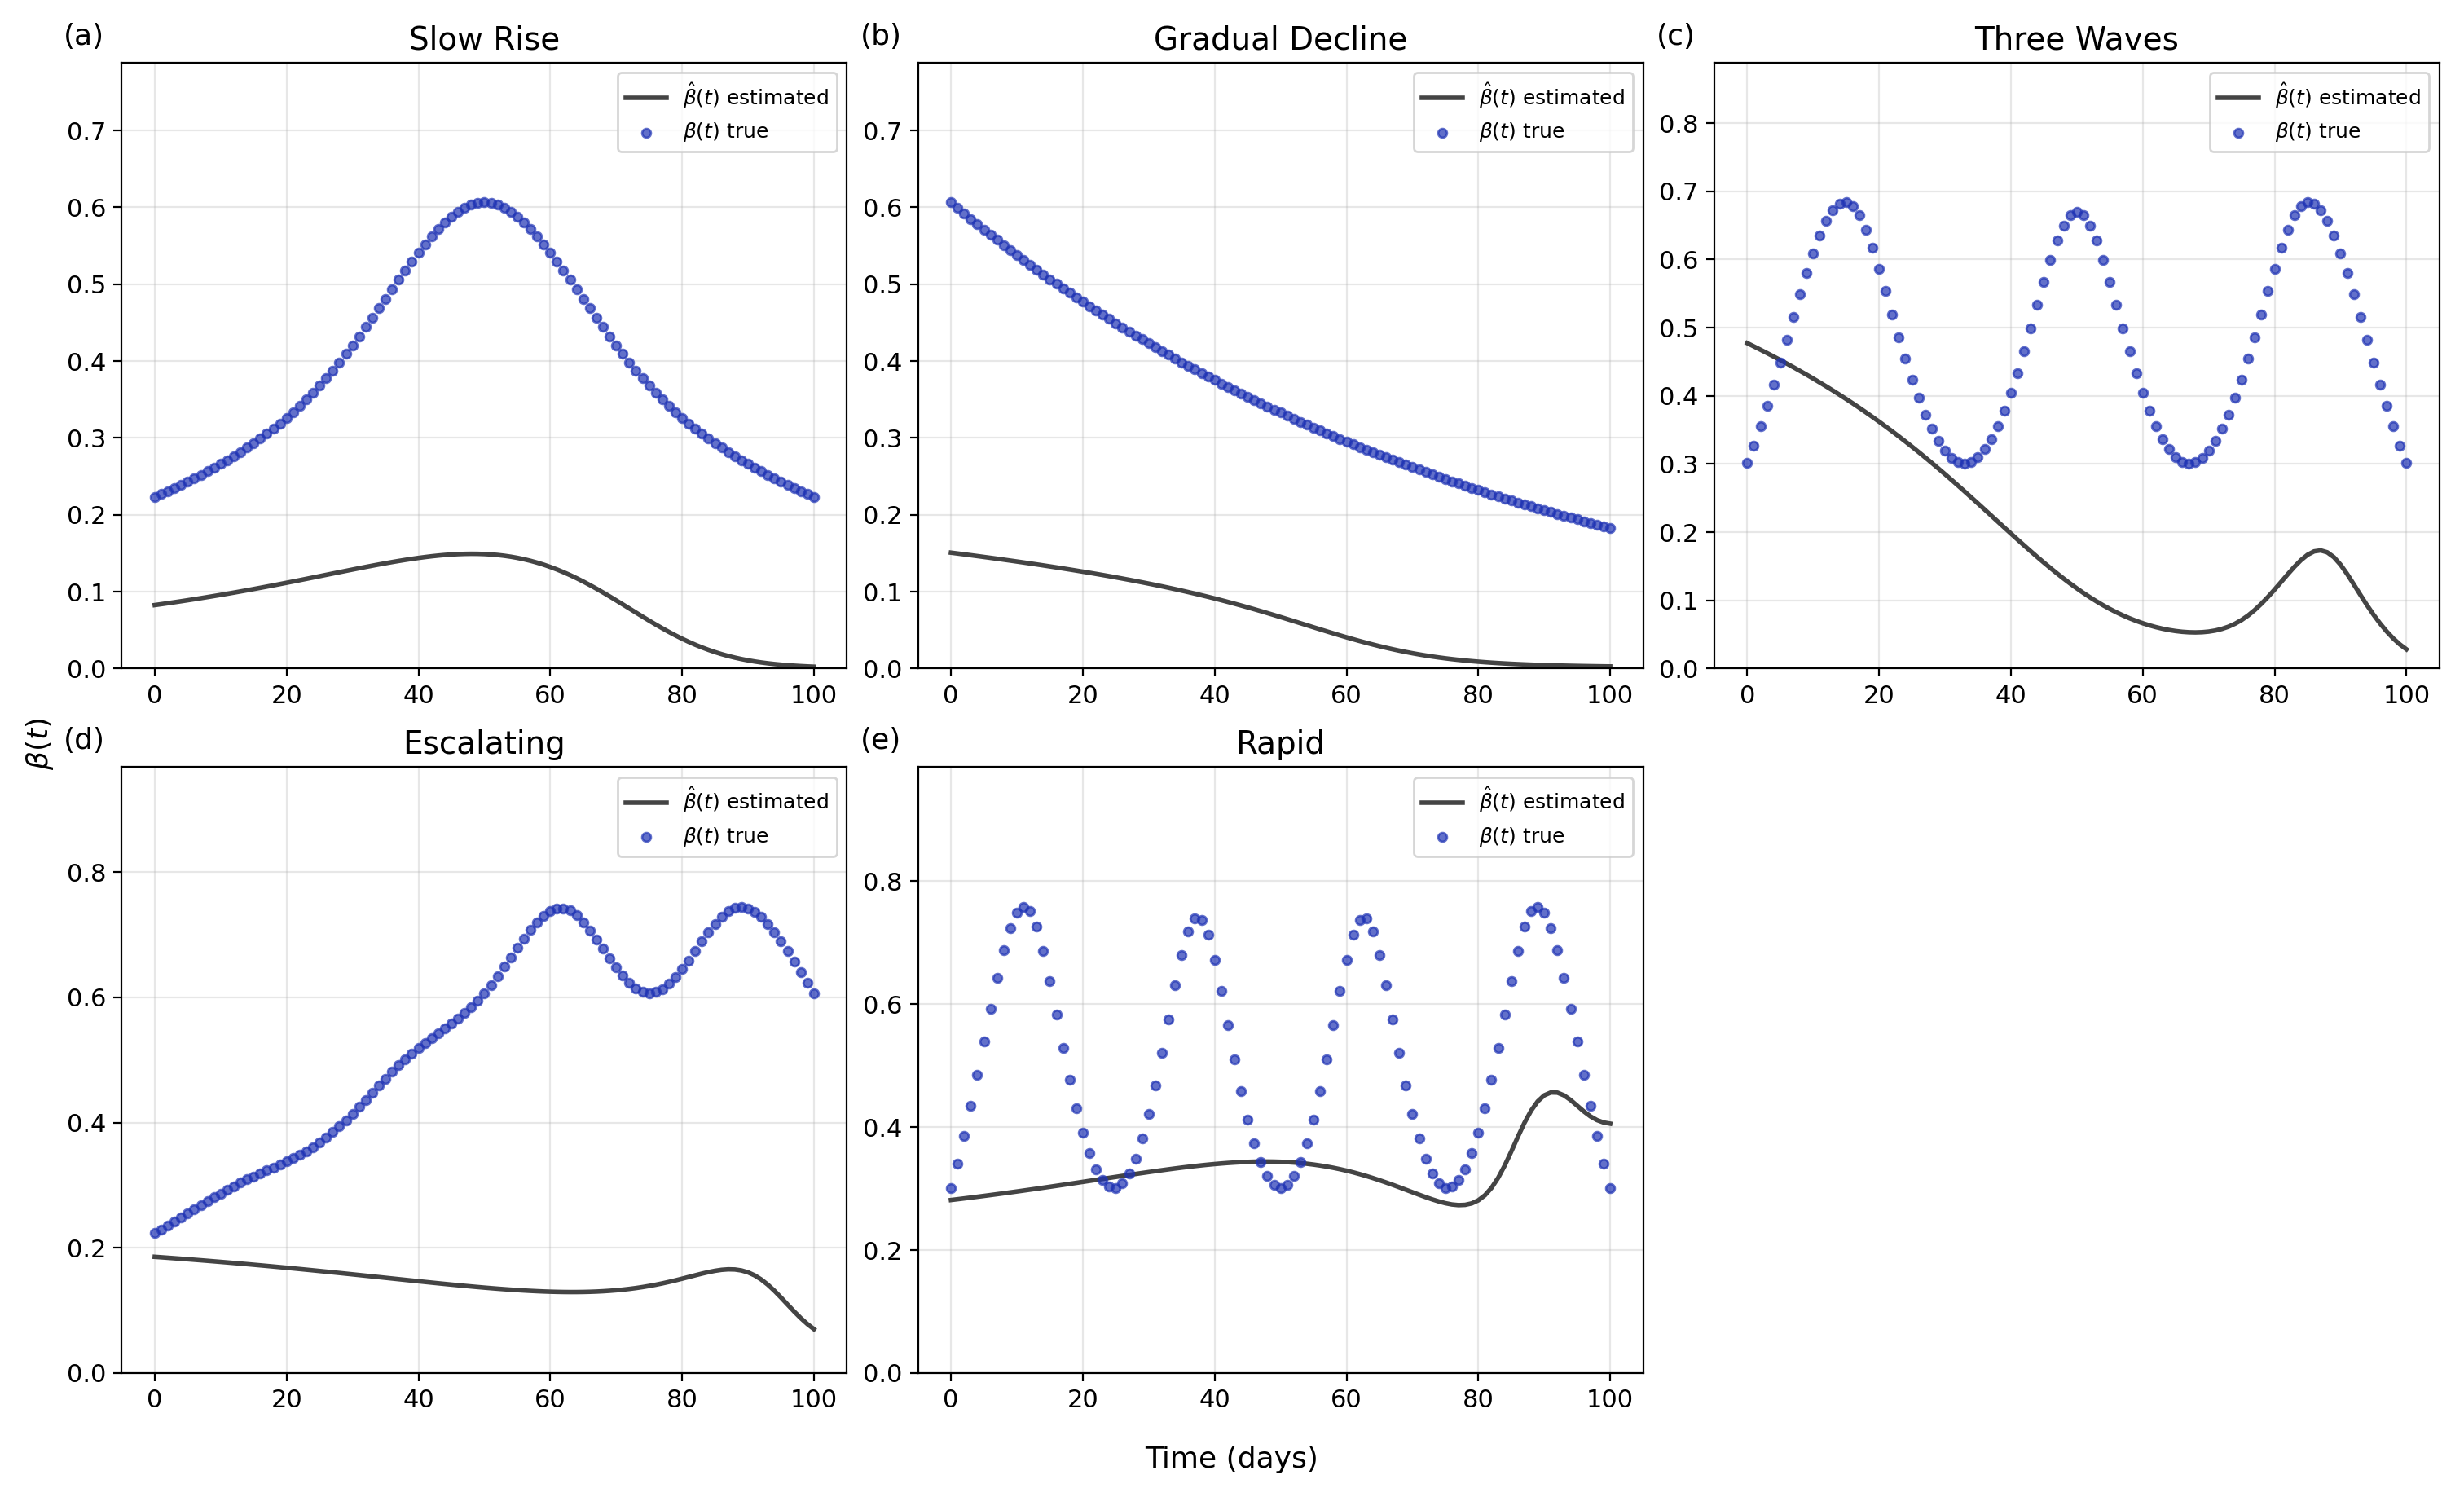
\includegraphics[width=1\linewidth]{figures/PINN_parameter_reconstruction_changing_beta_all_learnt_parameters.png}
    \caption{PINN parameter reconstruction on a range of time-varying beta transmission rate scenarios. (a) PINN parameter estimation when $\beta$ changes in the synthetic data as one wave that slowly rises and declines. (b) PINN parameter estimation when $\beta$ changes in the synthetic data as a gradual decline over time. (c) PINN parameter estimation when $\beta$ changes in the synthetic data as three waves. (d) PINN parameter estimation when $\beta$ changes in the synthetic data as increasing over time. (e) PINN parameter estimation when $\beta$ changes in the synthetic data as rapid oscillations. PINN provided with infection data only}
    \label{fig:PINN_parameter_estimation_changing_beta_infection_only}
\end{figure}


\subsection{Synthetic data generation: Gaussian observation noise}

After the SEIR model was developed, Gaussian observation noise ranging from 1\% to 20\% was added to the observed infections compartment (\cref{fig:syntheticdatanoise}).

\begin{figure}[H]
    \centering
    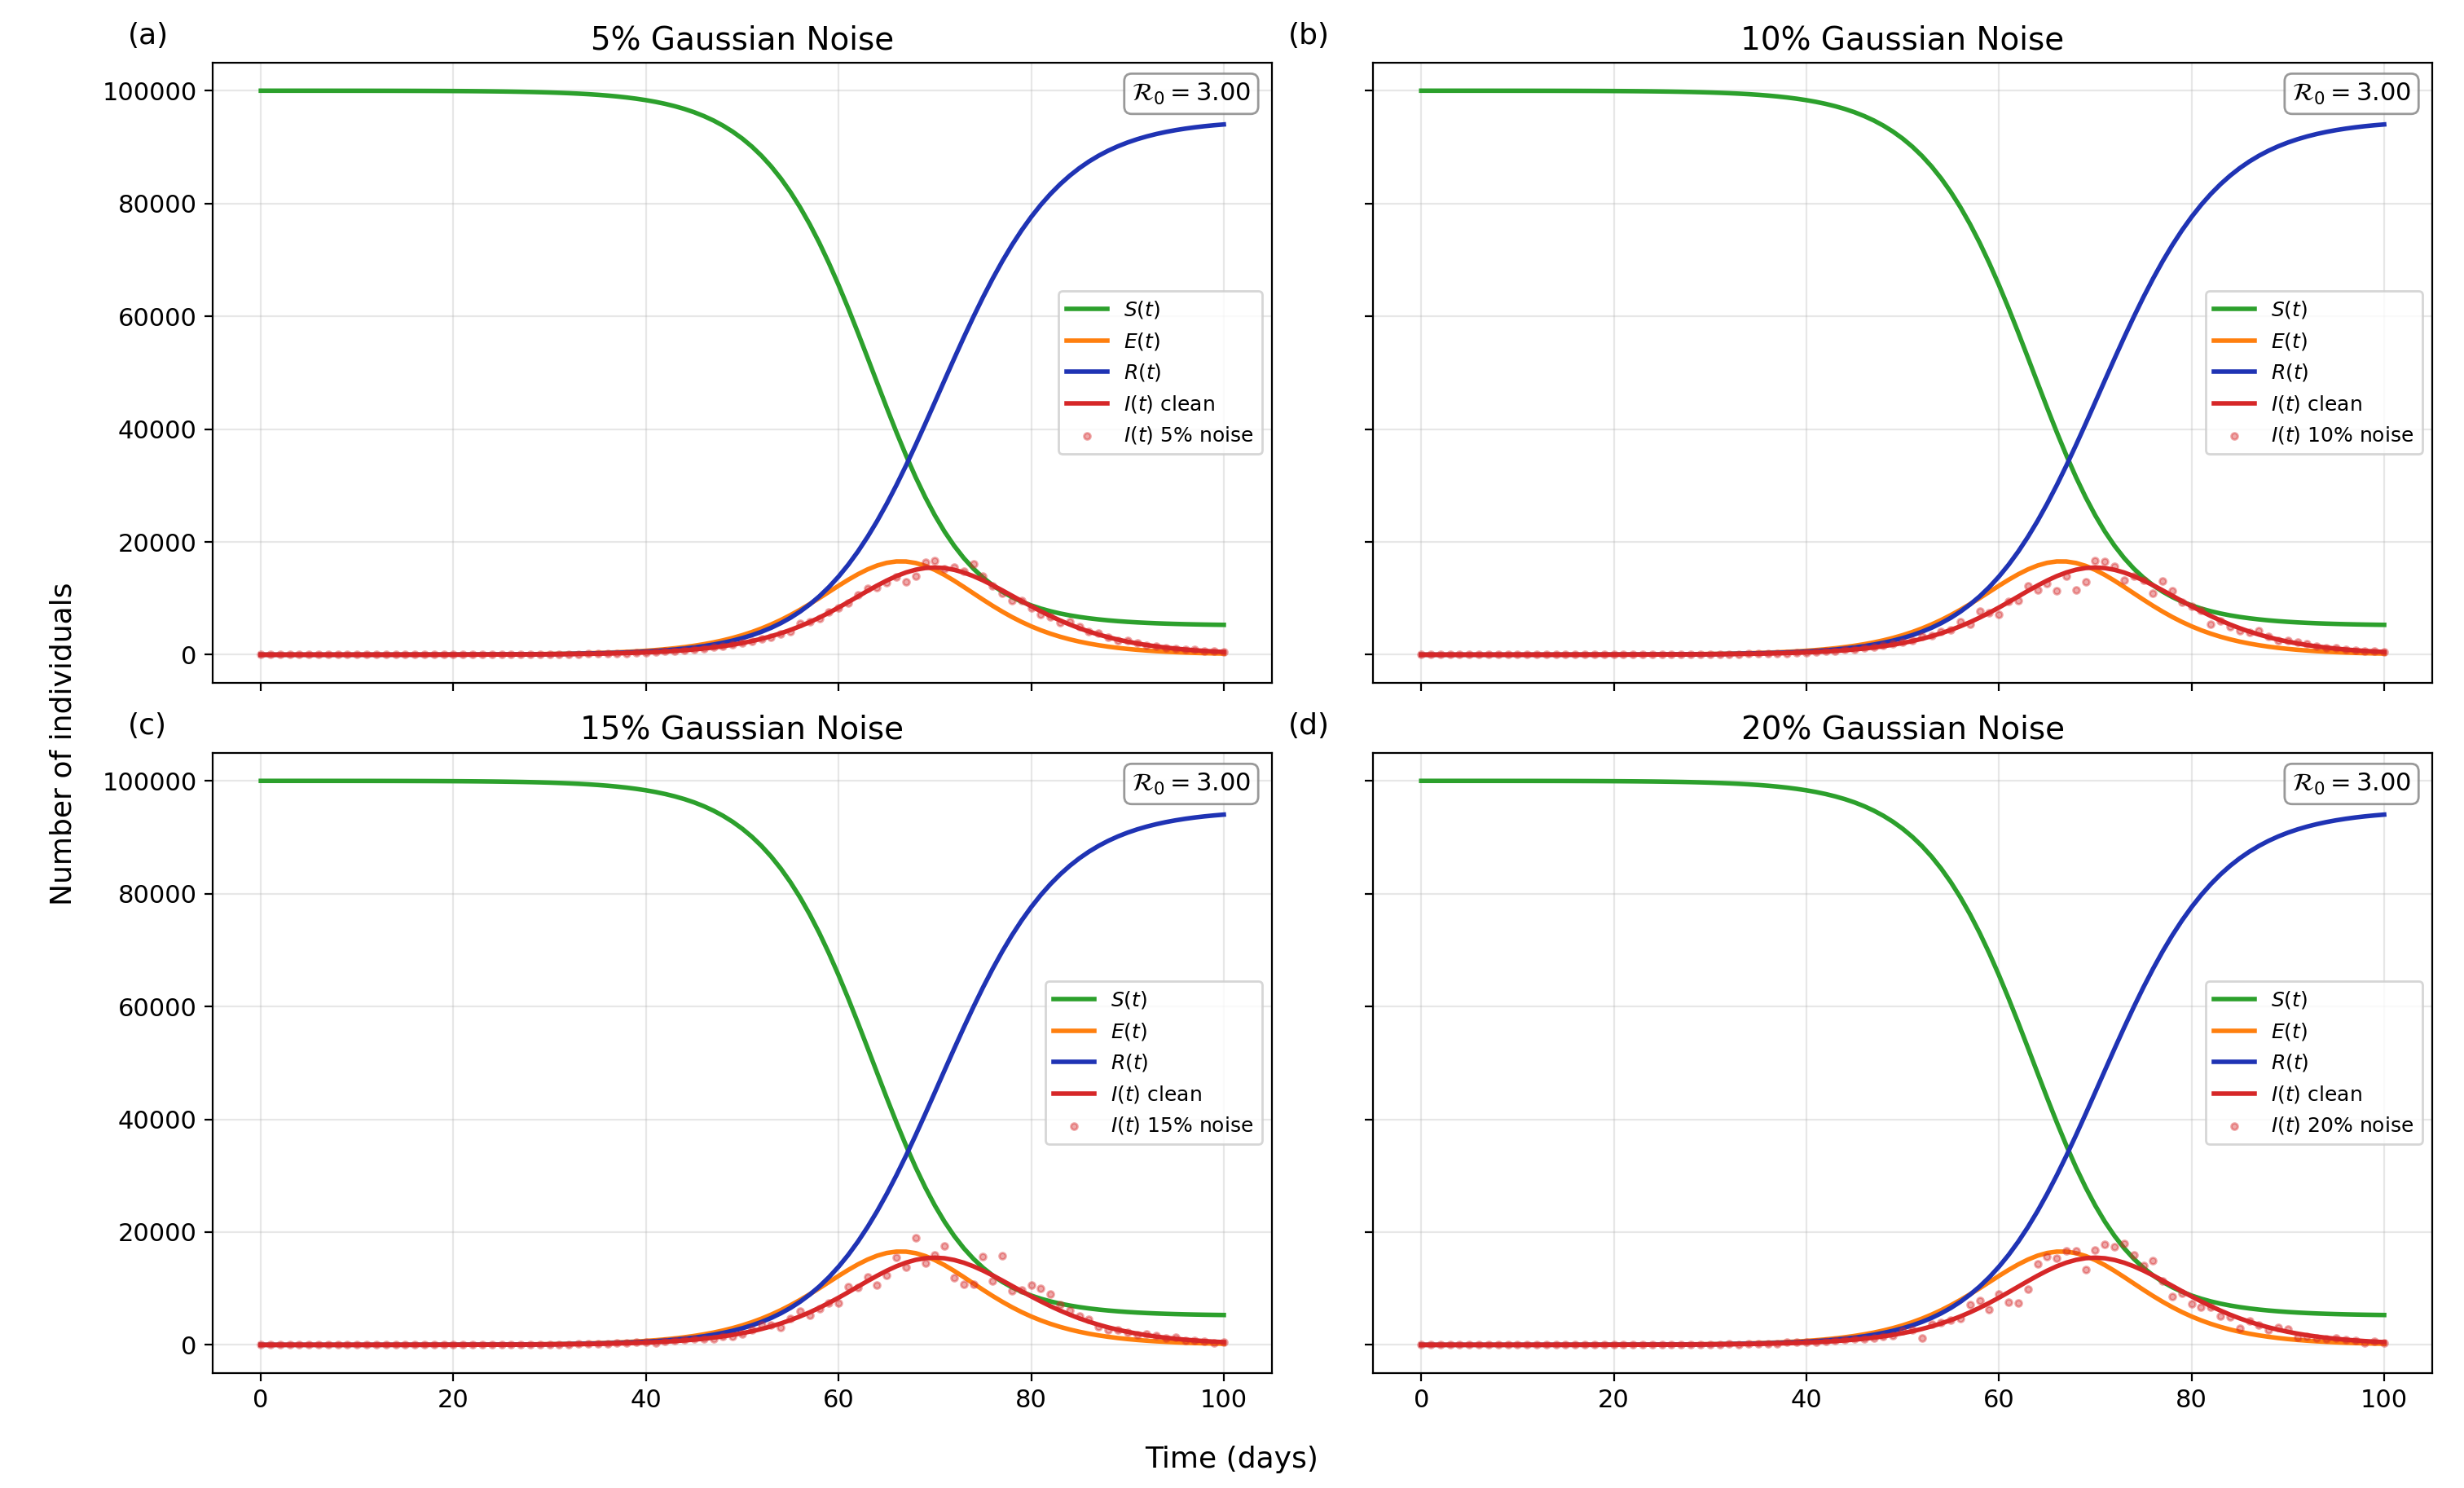
\includegraphics[width=1\linewidth]{figures/Synthetic_data_noise.png}
    \caption{Synthetic data simulations varying amounts of Gaussian observation noise added to the infected compartment of an SEIR model. (a) 5\% gaussian observation noise added to the infected compartment. (b) 10\% gaussian observation noise added to the infected compartment. (c) 15\% gaussian observation noise added to the infected compartment. (d) 20\% gaussian observation noise added the infected compartment.}
    \label{fig:syntheticdatanoise}
\end{figure}


\subsection{PINN forecasting: Gaussian observation noise, constant transmission rate, PINN provided with infection data, recovery rate and incubation period}

The PINN can provide accurate forecasts when gaussian observation noise is added to the infected compartment and the PINN is provided with infection data, recovery rate and incubation period. The PINN does not overfit the noise and can handle noise from 5-20\% (\cref{fig:PINN_forecasting_gaussian_noise_sigma_gamma_provided}). 

\begin{figure}[H]
    \centering
    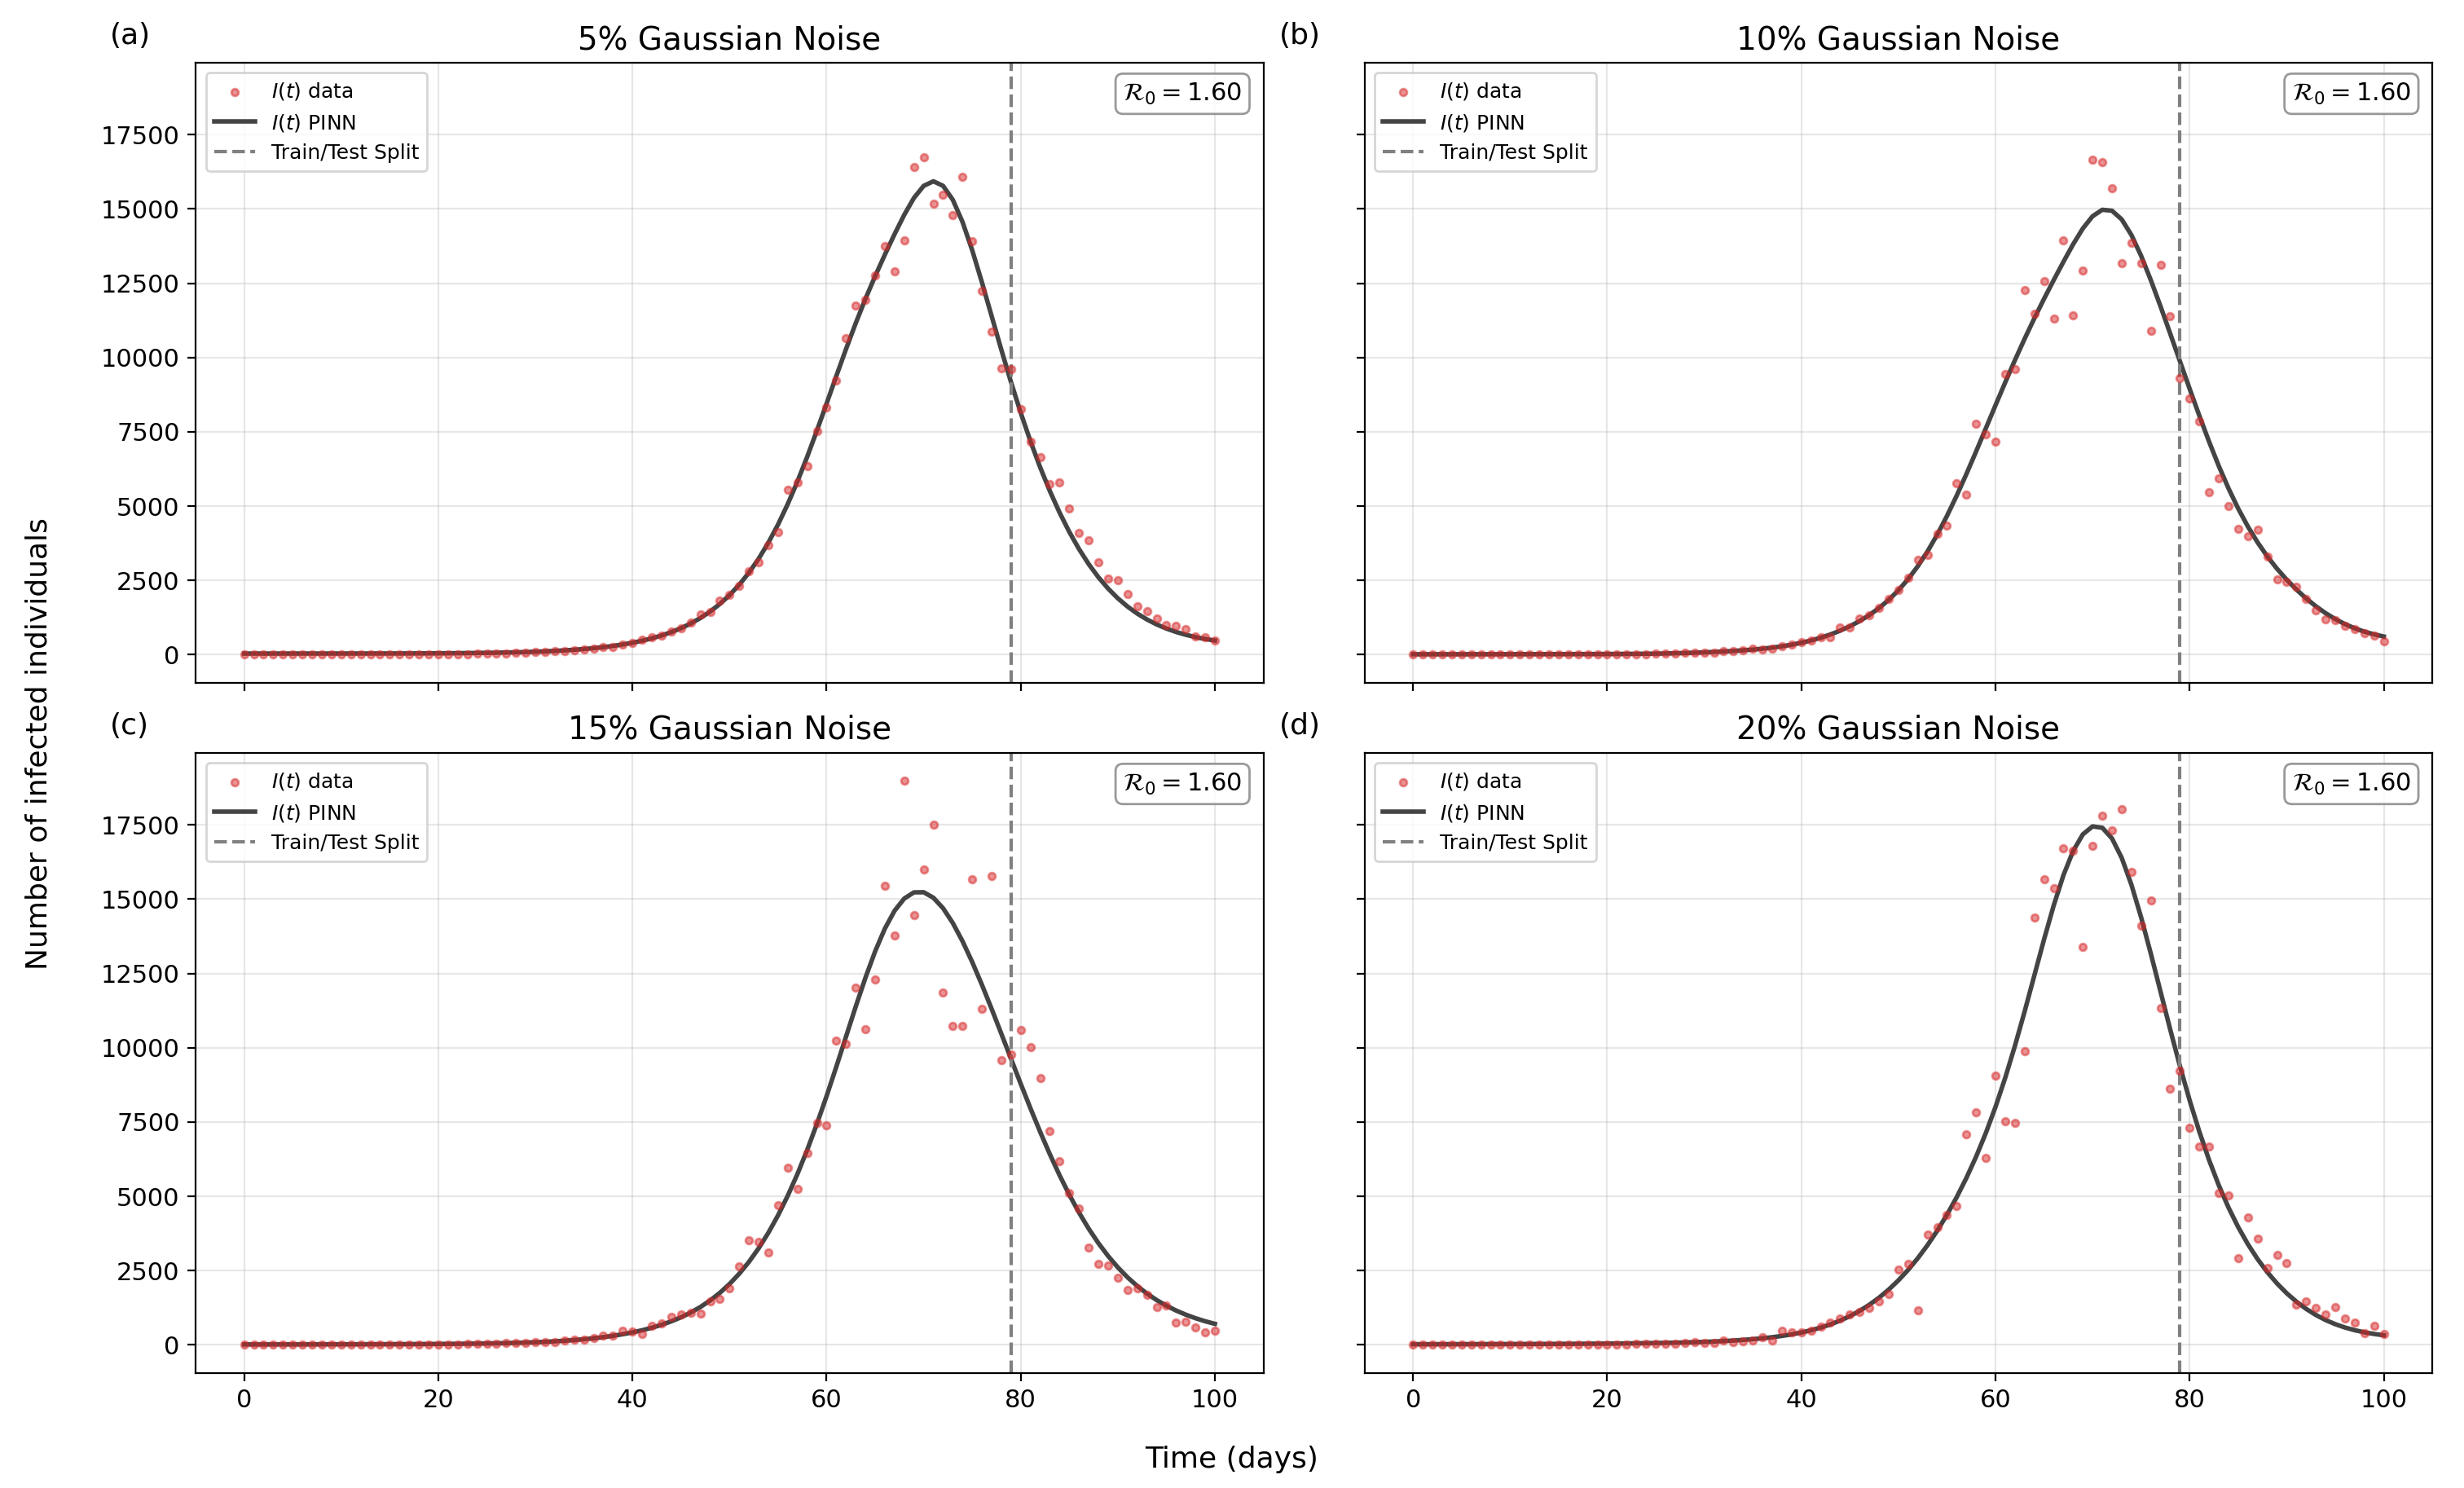
\includegraphics[width=1\linewidth]{figures/PINN_forecasting_gaussian_noise_sigma_gamma_provided.png}
    \caption{PINN forecasting the number of infections when varying levels of gaussian noise is added to the infected cases following the development of an SEIR model and the PINN was provided with case data, incubation period parameter and recovery rate parameter. (a) Forecasting when 5\% gaussian observation noise was added to the infected compartment. (b) Forecasting when 10\% gaussian observation noise was added to the infected compartment. (c) Forecasting when 15\% gaussian observation noise was added to the infected compartment. (d) Forecasting when 20\% gaussian observation noise was added to the infected compartment. The data was split 80\% for training, 20\% for testing.}
    \label{fig:PINN_forecasting_gaussian_noise_sigma_gamma_provided}
\end{figure}


\subsection{PINN forecasting: Gaussian noise, constant transmission rate, PINN provided with infection data only}

The PINN can provide accurate forecasts when gaussian observation noise is added to the infected compartment until 15\% of gaussian observation noise is added and the PINN is provided with infection data only (\cref{fig:PINN_forecasting_gaussian_noise_all_learnable}).

\begin{figure}[H]
    \centering
    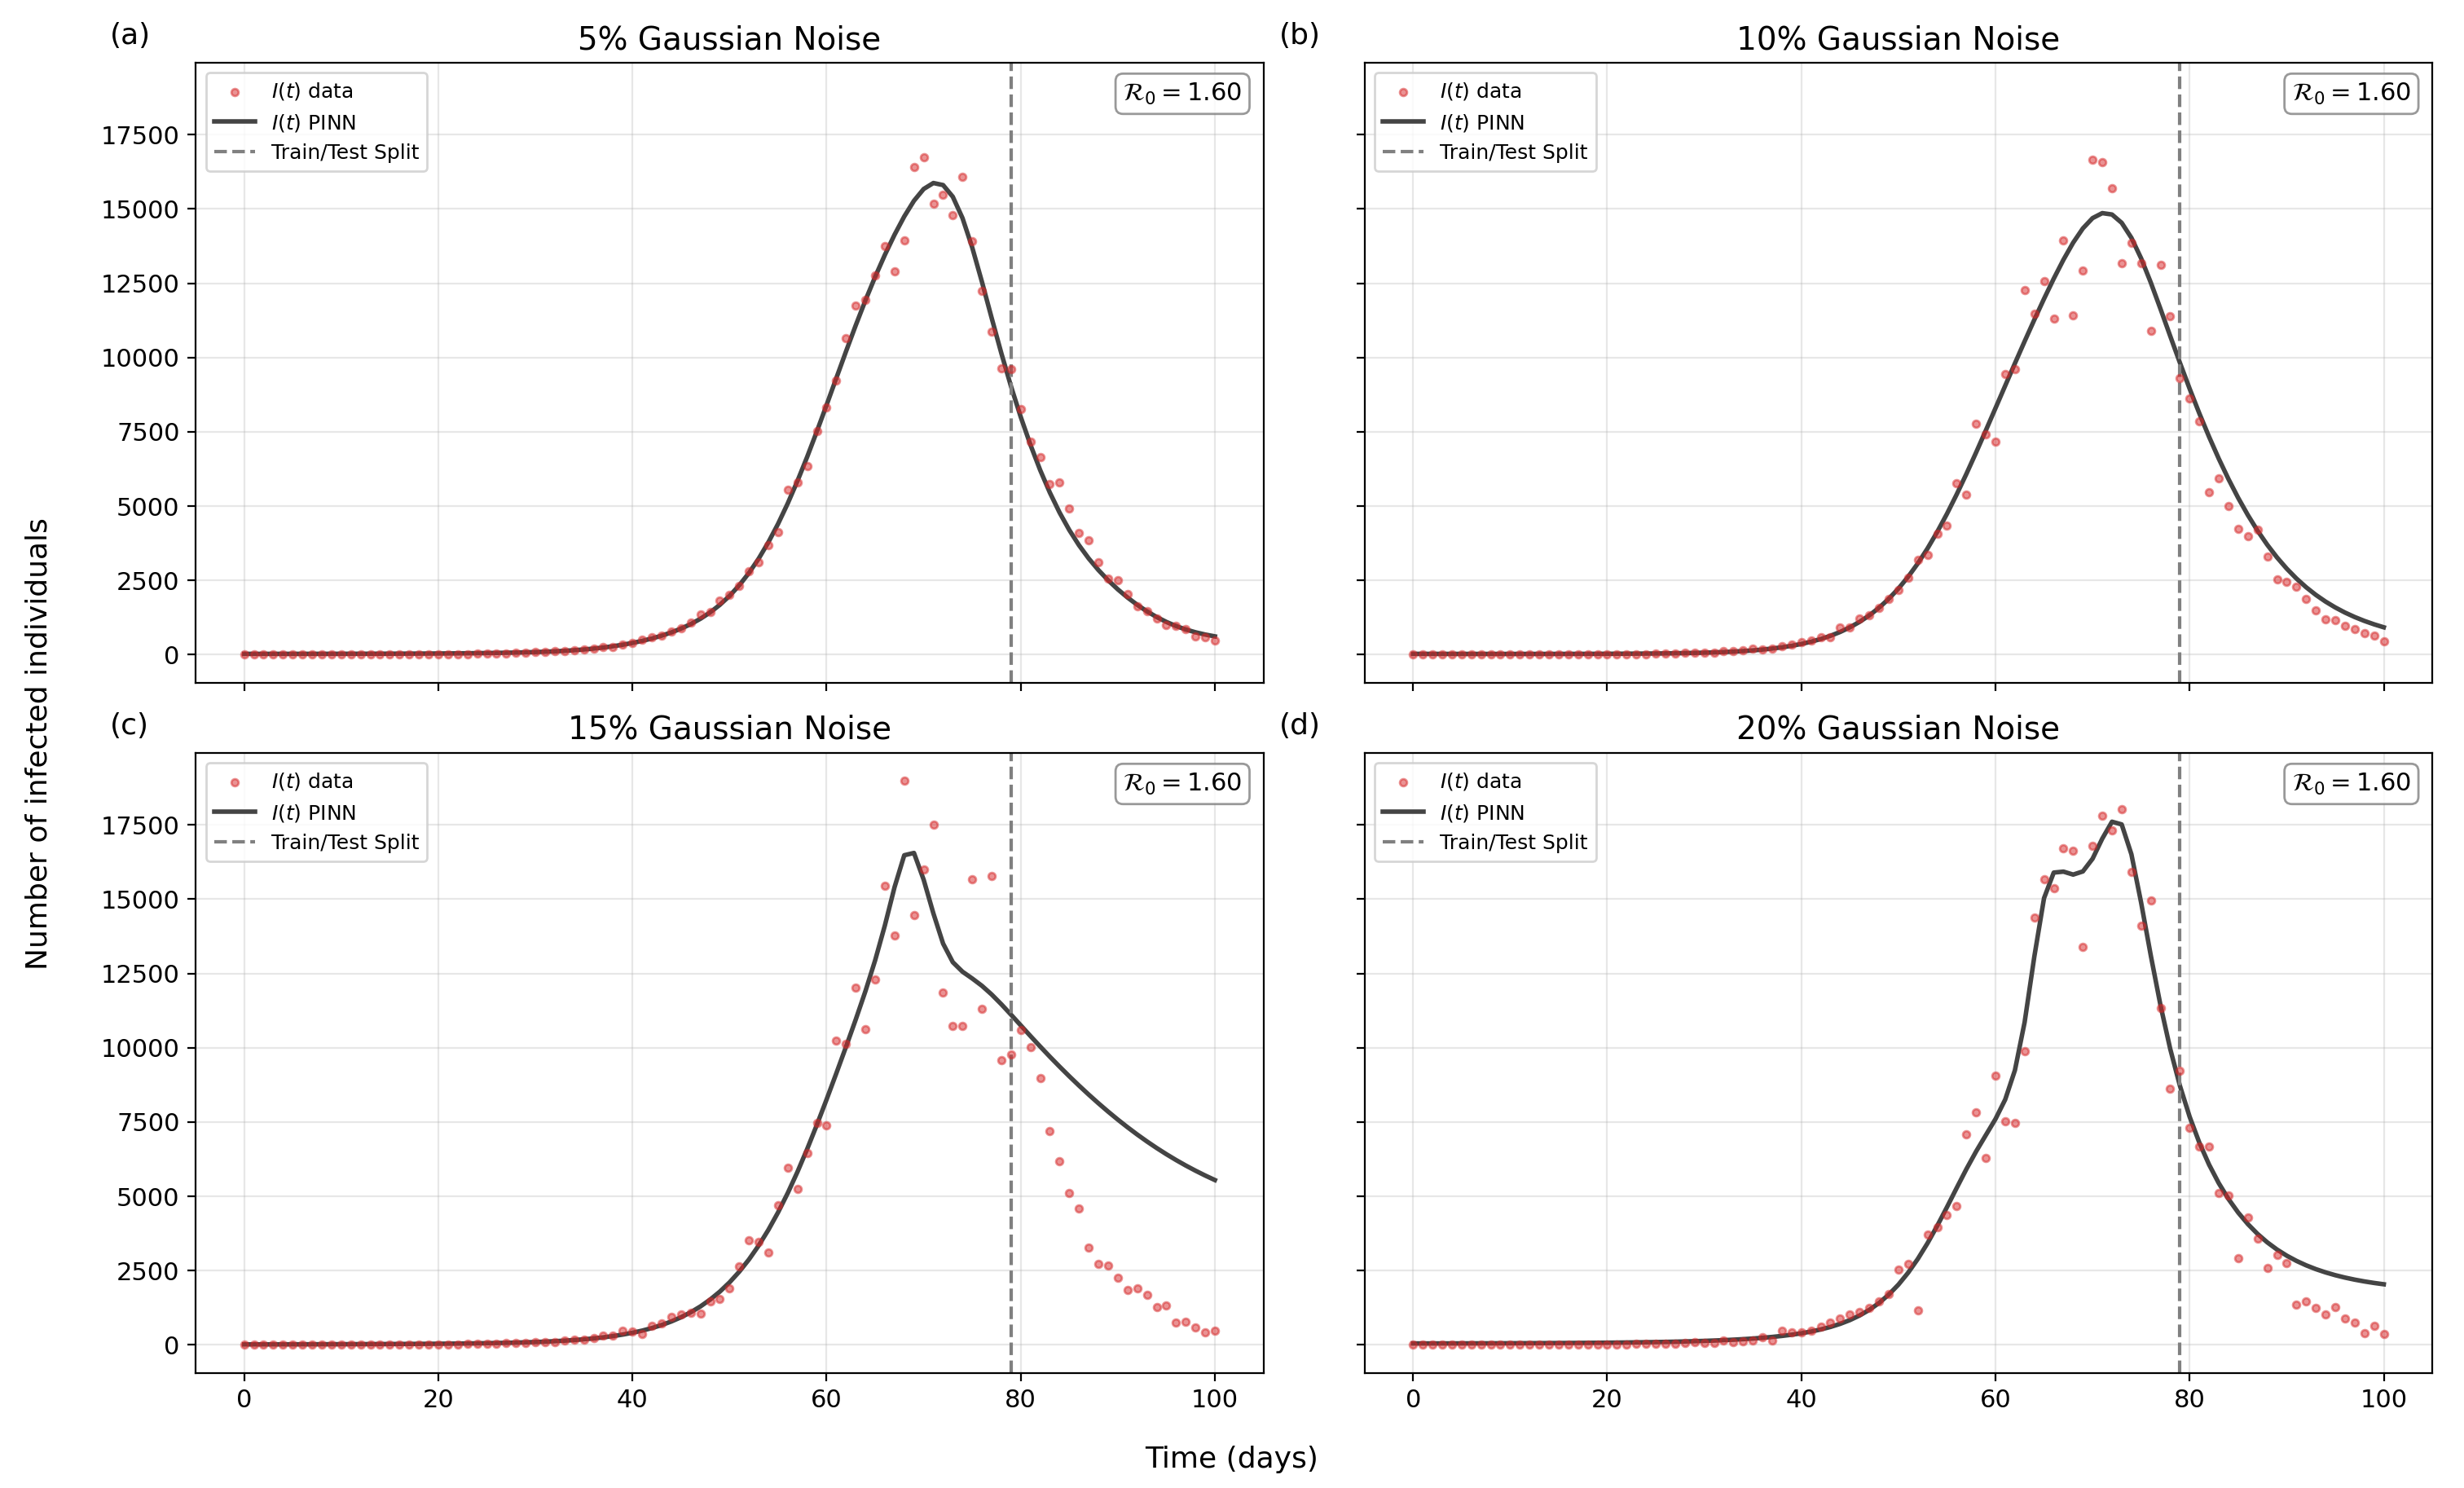
\includegraphics[width=1\linewidth]{figures/PINN_forecasting_gaussian_noise_all_learnable.png}
    \caption{PINN forecasting the number of infections when varying levels of gaussian noise is added to the infected cases following the development of an SEIR model and the PINN was provided with infection data only. (a) Forecasting when 5\% gaussian observation noise was added to the infected compartment. (b) Forecasting when 10\% gaussian observation noise was added to the infected compartment. (c) Forecasting when 15\% gaussian observation noise was added to the infected compartment. (d) Forecasting when 20\% gaussian observation noise was added to the infected compartment. The data was split 80\% for training, 20\% for testing.}
    \label{fig:PINN_forecasting_gaussian_noise_all_learnable}
\end{figure}

\subsection{PINN parameter reconstruction: Gaussian noise, constant transmission rate, PINN provided with infection data, recovery rate and incubation period}

The PINN struggled to reconstruct the transmission rate parameter when gaussian observation noise was added to the infected compartment following SEIR model development (\cref{fig:parameterrecoverygaussiannoise}). 

In these scenarios, despite $\beta$ being structurally identifiable from the SEIR model, it is not practically identifiable (identifiable from the noisy measurements available) \parencite{Pant2026}. 

\begin{figure}[H]
    \centering
    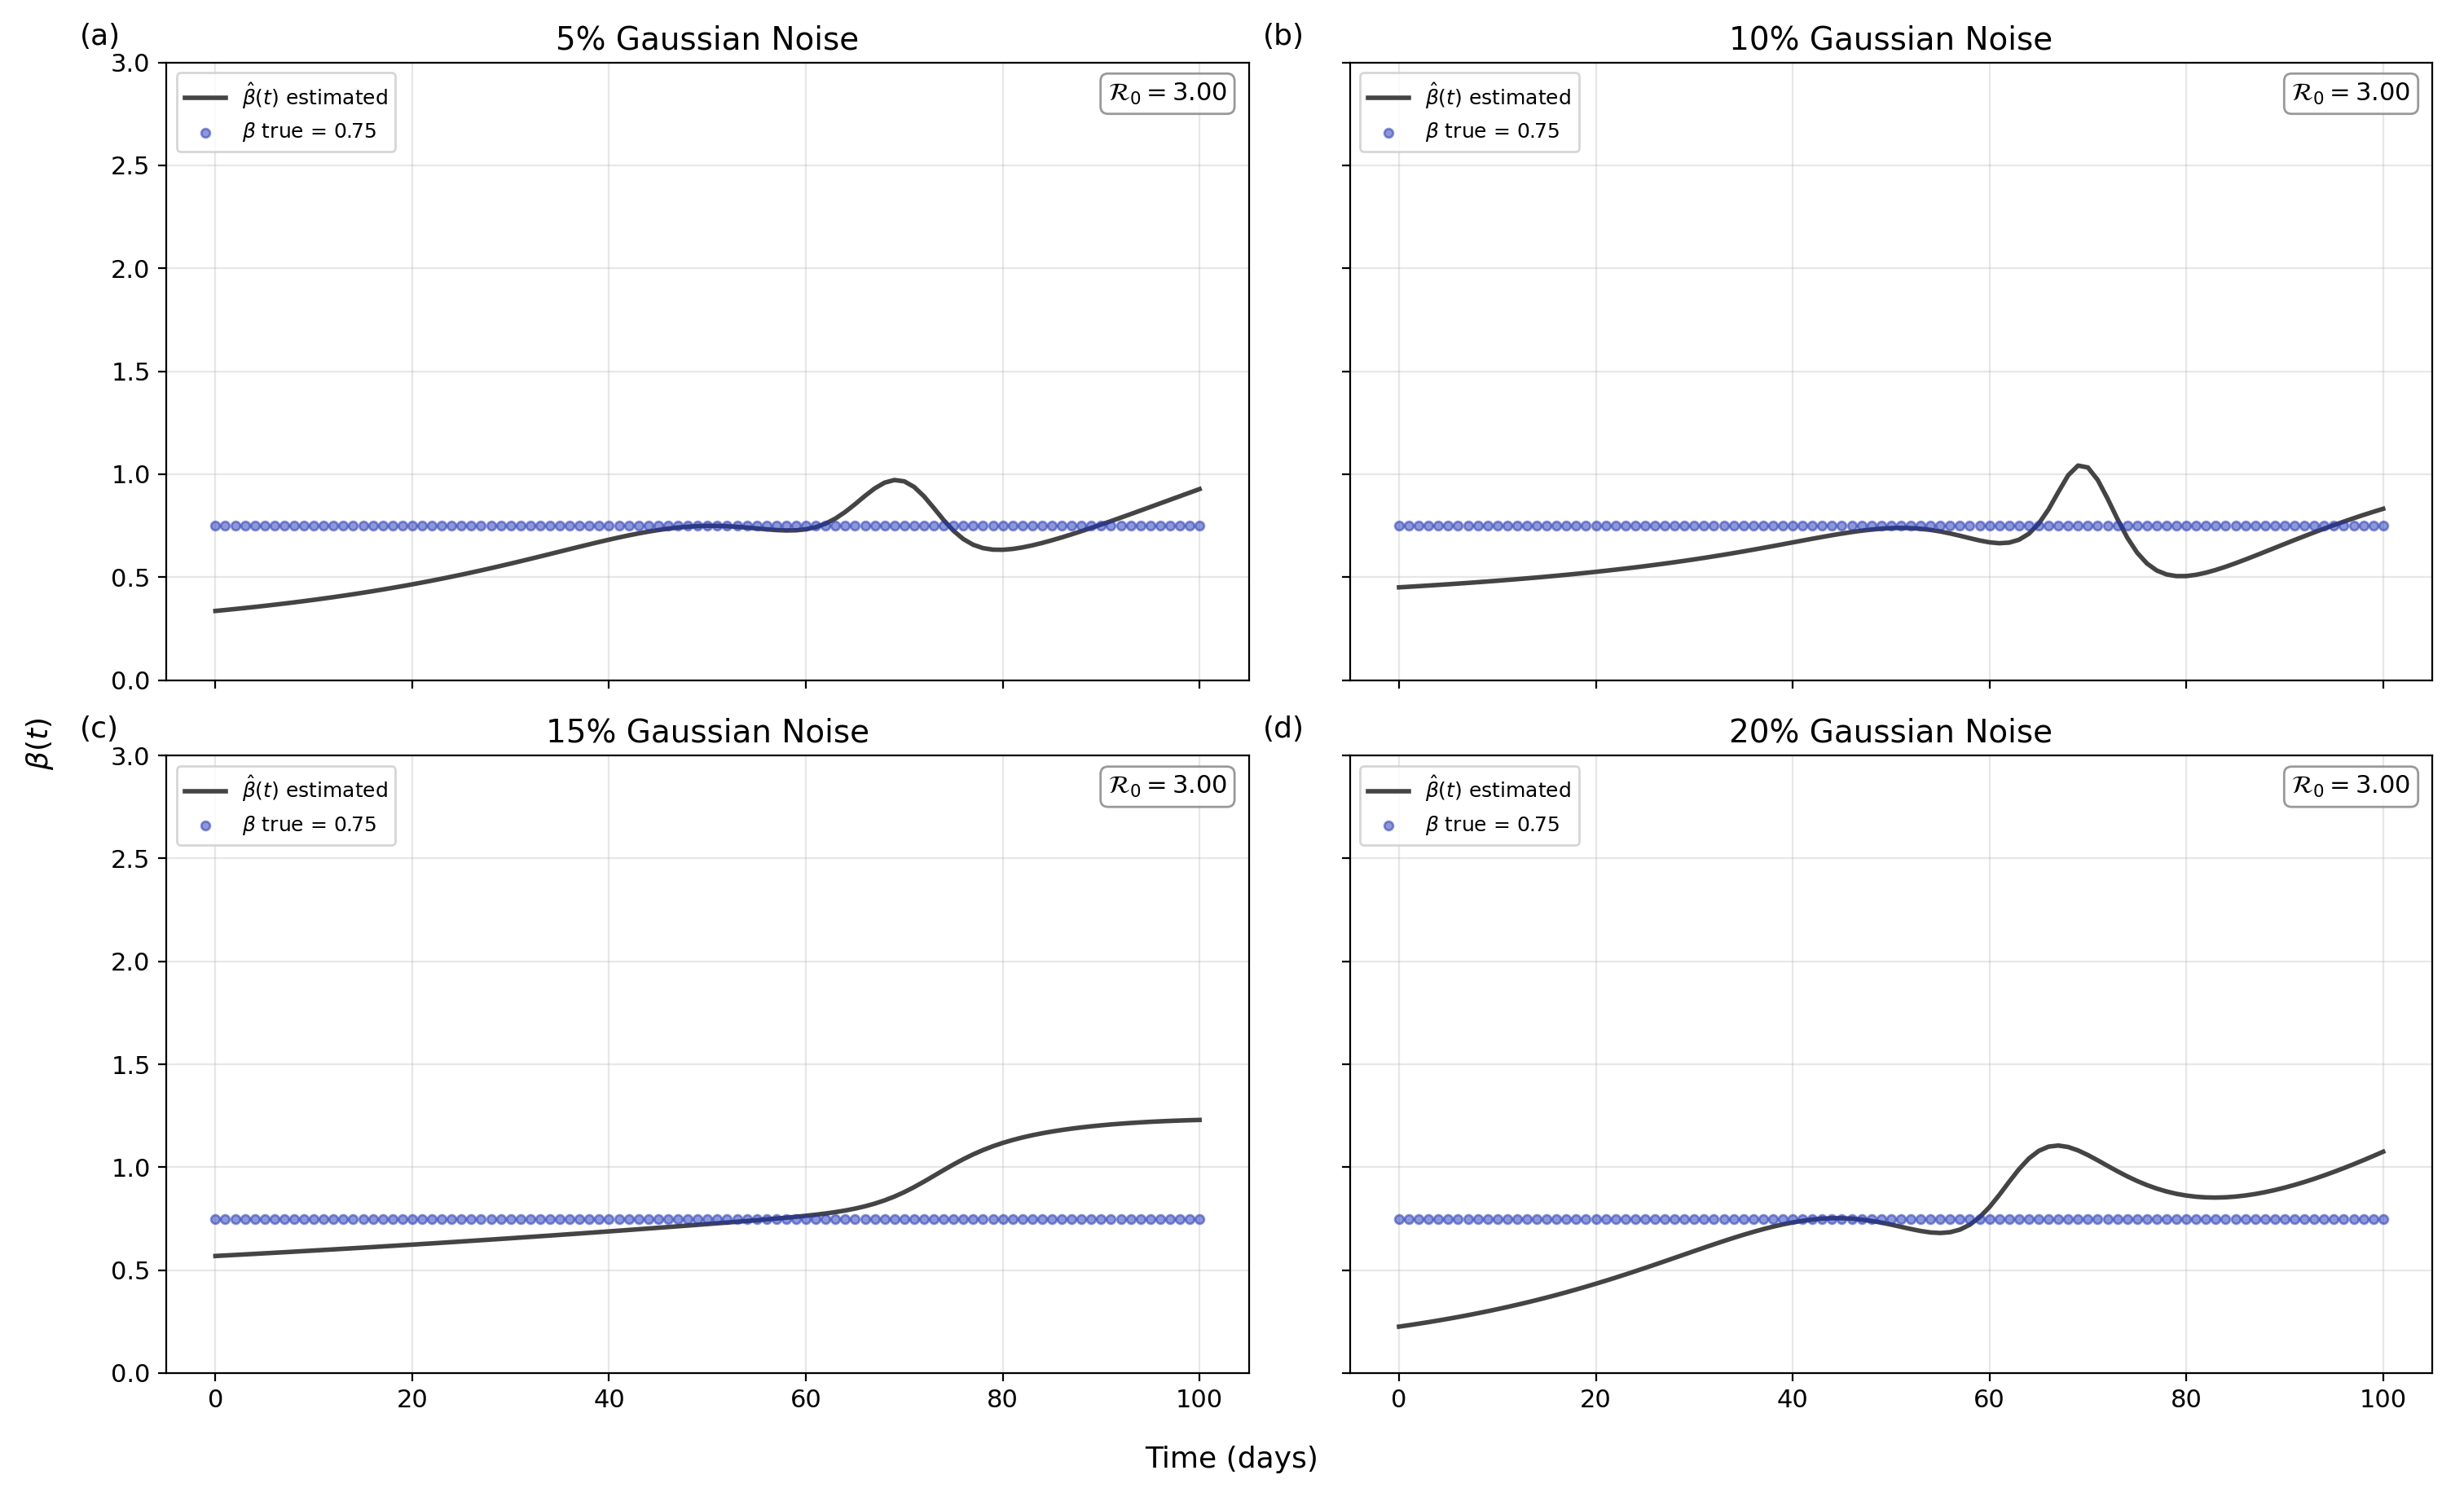
\includegraphics[width=1\linewidth]{figures/PINN_gaussian_noise_parameter_reconstruction.png}
    \caption{PINN transmission rate reconstruction when varying levels of gaussian noise is added to the infected cases following the development of an SEIR model and the PINN was provided with case data, incubation period parameter and recovery rate parameter. (a) Transmission rate reconstruction when 5\% gaussian observation noise was added to the infected compartment. (b) Transmission rate reconstruction when 10\% gaussian observation noise was added to the infected compartment. (c) Transmission rate reconstruction when 15\% gaussian observation noise was added to the infected compartment. (d) Transmission rate reconstruction when 20\% gaussian observation noise was added the infected compartment.}
    \label{fig:parameterrecoverygaussiannoise}
\end{figure}

\subsection{PINN parameter reconstruction: Gaussian noise, constant transmission rate, PINN provided with infection data only}

The PINN failed to reconstruct the transmission rate parameter when gaussian observation noise was added to the infected output of the SEIR model and the PINN was provided with infection data only (\cref{fig:parameterrecoverygaussiannoisinfectiononly}).

\begin{figure}[H]
    \centering
    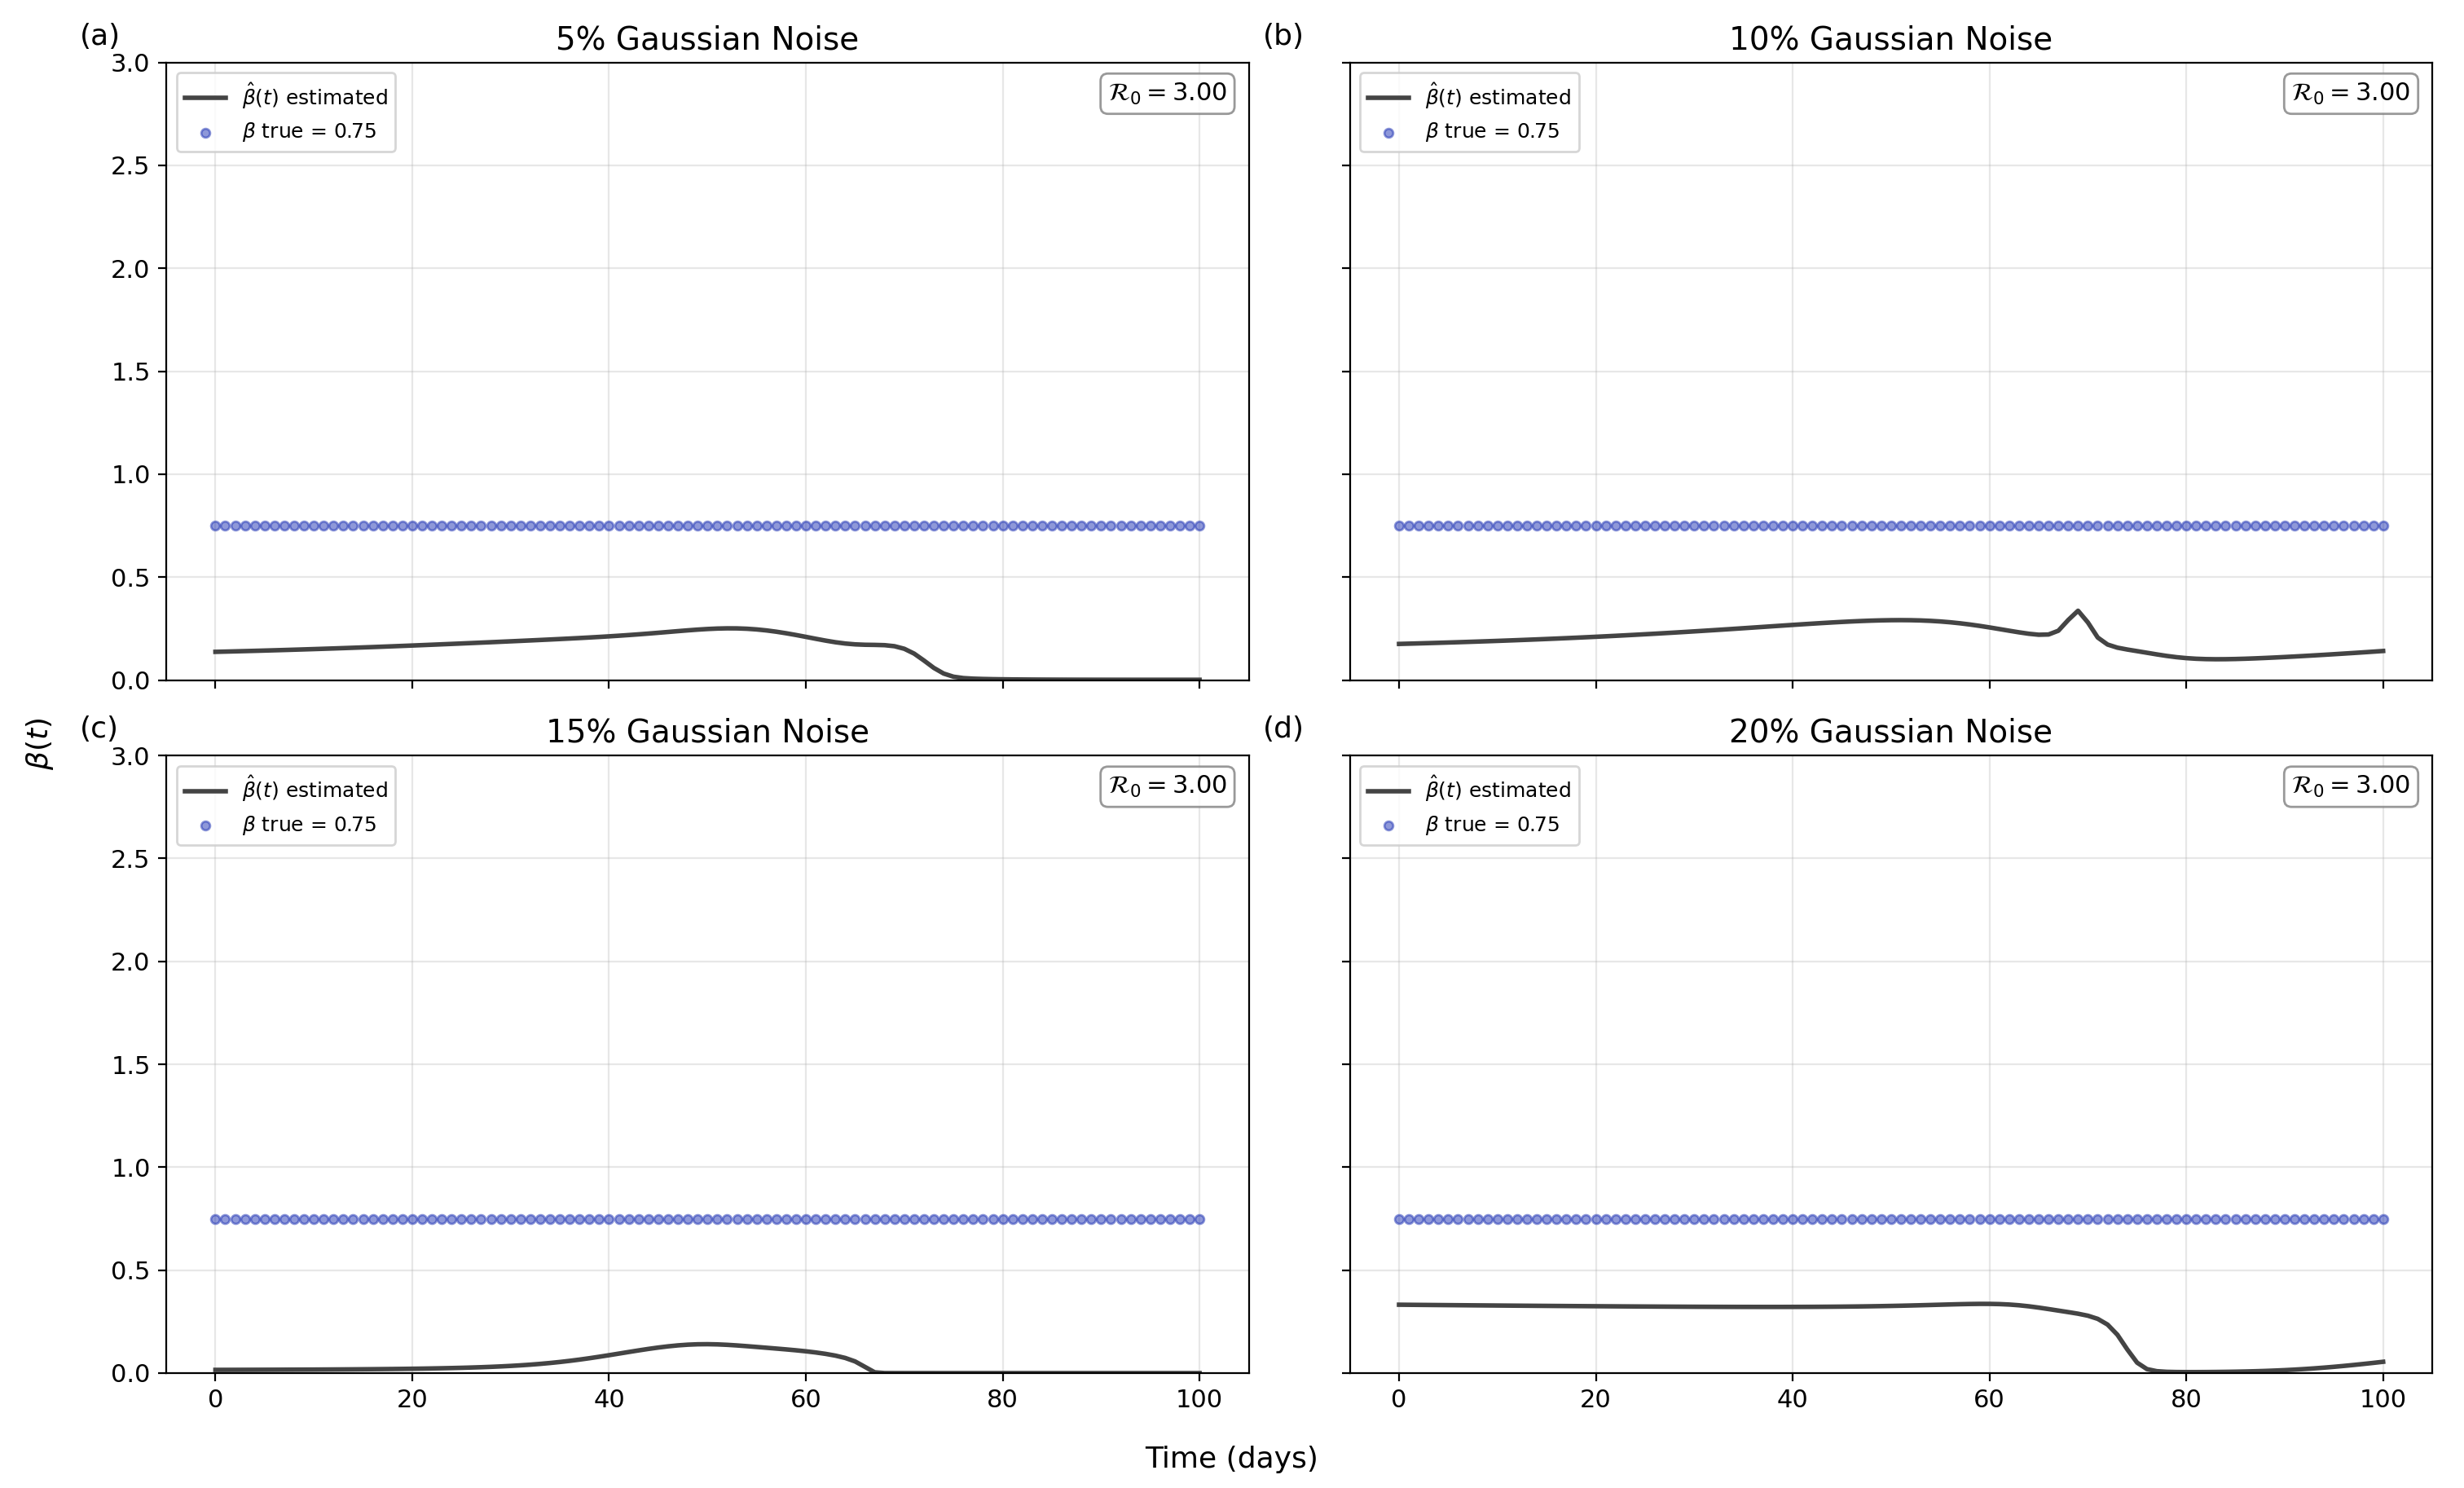
\includegraphics[width=1\linewidth]{figures/PINN_parameter_gaussian_noise_all_learnable_parameters.png}
    \caption{PINN transmission rate reconstruction when varying levels of gaussian noise is added to the infected cases following the development of an SEIR model and the PINN was provided with infection data only. (a) Transmission rate reconstruction when 5\% gaussian observation noise was added to the infected compartment. (b) Transmission rate reconstruction when 10\% gaussian observation noise was added to the infected compartment. (c) Transmission rate reconstruction when 15\% gaussian observation noise was added to the infected compartment. (d) Transmission rate reconstruction when 20\% gaussian observation noise was added the infected compartment.}
    \label{fig:parameterrecoverygaussiannoisinfectiononly}
\end{figure}


\subsection{UKHSA COVID-19 case data England}

PINN trained on data from July 2020 – April 2022
Rolling window approach
Initial training on weeks 1 – 17 with predictions for weeks 18 to 21
Training window then shifted by one week
Model trained on weeks 1 – 18 and forecasting weeks 19 – 22
Repeated for all 93 weeks

\subsection{Synthetic data generation: metapopulation SEIR model}
Synthetic data was generated for the metapopulation PINN. 5 patches were modelled each with varying transmission rates from 0.6 - 0.8. The recovery rate ($\gamma$) was 0.25 and the incubation rate ($\sigma$) was 0.25, corresponding to a mean infectious period and mean incubation period of 4 days (\cref{fig:metapopulation}.

\begin{figure}[H]
    \centering
    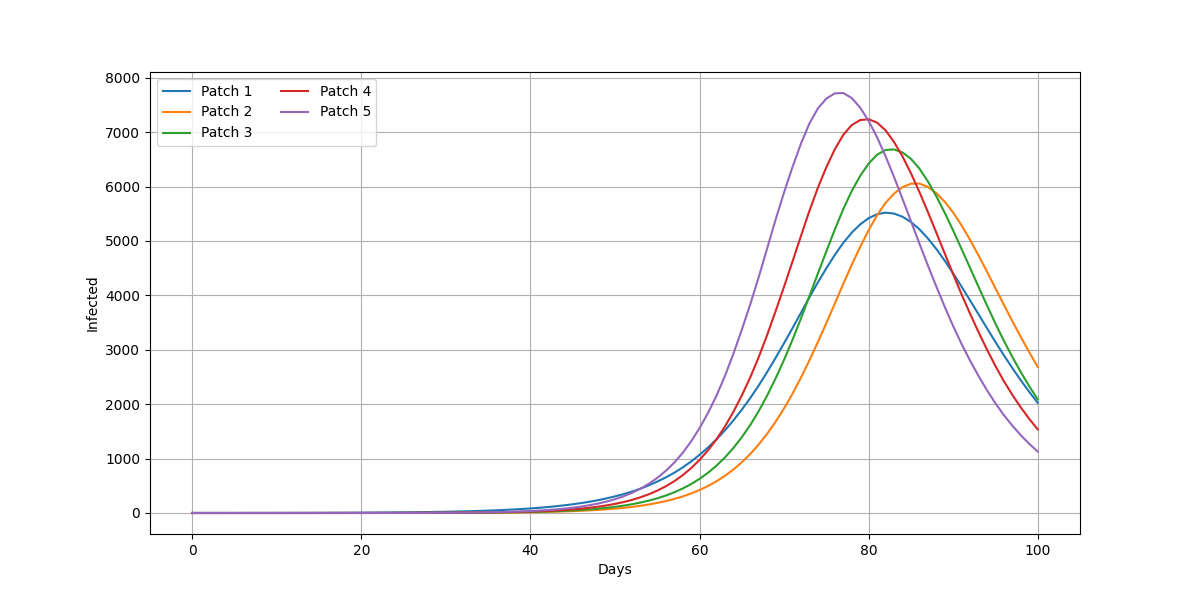
\includegraphics[width=1\linewidth]{figures/metapopulation.png}
    \caption{Synthetic data for metapopulation SEIR model.}
    \label{fig:metapopulation}
\end{figure}



\section{Discussion/future directions}

\begin{itemize}
    \item Testing the model on more real-world epidemiological data e.g. RKI data \href{}{https://github.com/bristol-vaccine-centre/rsurvstat}
    \item Multi-modal data integration e.g. hospitalisations, deaths, wastewater?
    \item Could embed more complex architectures e.g. transformer, LSTM
    \item Foundation multi-pathogen model? \parencite{Lau2026}
    \item Spatial PINN - embed metapopulation ODEs/graph neural network/PDEs
    \item Use an agent-based model for testing on more synthetic epidemiological data. Would allow testing on a wider range of epidemiological scenarios.
    \item Because incorporating space by a metapopulation model is conceptually similar to developing an age-structured model, an age structured PINN could be developed. Important for infections such as Varicella.
    \item Develop Bayesian PINN for uncertainty quantification
    \item Self adjusting PINN weights \parencite{https://doi.org/10.48550/arxiv.2009.04544}
    \item Symbolic regression on PINN outputs?
    \item Exploring fourier feature mapping for PINN to help with spectral bias? \parencite{Ning2023}
    \item Could use PINN to estimate true infections 
    
\end{itemize}


\subsection{Extending "Toward optimal disease surveillance with graph-based active
learning"}

PINN good at handling noisy and sparse data. When only one node is observed, PINN can handle data sparsity. PINN would also provide information on why locations need testing e.g. high importation risk due to proximity to outbreak. PINN advantage is in early stages of the model which as shown in the paper are important for small test budgets \parencite{Tsui2024}.



\printbibliography

\end{document}
